%%Allgeimeine Vorlage

%Artikel auf A4 Papier
\documentclass[12pt, a4paper]{article} 
 
\newcommand{\doctitle}
{ATFrogs - Handbuch}
 
%Deutsche Sprache, Silbentrennung, Grafikeinbindung
%Umlaute k{\"o}nnen direkt eingegeben werden
\usepackage[T1]{fontenc}
\usepackage[latin1]{inputenc}
\usepackage{ngerman}
\usepackage{times} 
\usepackage{mathptm}
\usepackage{fancyhdr}
\usepackage{makeidx}
\usepackage{longtable}

\usepackage{listings}

%%Erzwingt Ausgabe von Glossar- und Index-Dateien: anfdef.idx und anfdef.glo
\makeindex
\makeglossary
\renewcommand{\indexname}{}




%%Layout der Kopfzeile.
%\pagestyle{fancy} 
%\fancyhead[R]{\thepage}
%\fancyfoot[C]{}

\title{\doctitle}

%%Wenn pdflatex(f{\"u}r pdf-Dateien) verwendet wird, dann diese Zeile Verwenden
\usepackage[pdftex]{graphicx}
\usepackage{times}

\usepackage{textcomp} % u.a. TM-Zeichen
\usepackage{url}

\tolerance=10000 % Toleranz beim Trennen
% Disable single lines at the start of a paragraph (Schusterjungen)
\clubpenalty = 10000
%
% Disable single lines at the end of a paragraph (Hurenkinder)
\widowpenalty = 10000 \displaywidowpenalty = 10000

\newcommand{\TODO}[1]{ $\star \star \star$ \textbf{ TODO:  #1 }  $\star \star \star$}


\newcommand{\ICON} [1] { \includegraphics[scale=0.5] {#1} }
\newcommand{\ATFROGS}{\textit{ATFrogs}\ }
\newcommand{\ATFROGSnosp}{\textit{ATFrogs}}
\newcommand{\OPENXCHANGEsp}{\textit{Open-XChange}\texttrademark\ }
\newcommand{\OPENXCHANGE}{\textit{Open-XChange}\texttrademark}

\usepackage{color}
\newcommand{\NOTE}[1]{
    \hspace*{1cm}
    \fcolorbox{white}{red}{\fcolorbox{red}{white}{\parbox{0.8\textwidth}{
    	\textcolor{red}{{\sffamily \small \textbf{Hinweis:}}}\\
    	{\sffamily \textit{#1}}
    \hspace*{1cm}
    }}}
}

\usepackage[top=2.5cm, bottom=2.5cm, left=3.5cm, right=2.5cm]{geometry}


%%Layout der Kopfzeile.

\pagestyle{fancy}

\fancyhead[R]{\thepage}

\fancyfoot[C]{\ATFROGS Handbuch - August 2005}
%\begin{minipage}{1.5cm}
%\vspace{-1em}
%\includegraphics[width=1.5cm]{atfrogsicon}
%\end{minipage}




%%Wenn latex(f{\"u}r dvi/ps-Dateien) verwendet wird, dann diese Zeile Verwenden
%\usepackage[dvips]{graphicx}


%%Das brauchen wir, damit alle Zeilen ganz links anfangen
\setlength{\parindent}{0pt}

%%Hier m{\"u}ssen Name und Titel angepasst werden
\title{Handbuch}
\author{Gebhardt \and van Hoorn}

%Bei zwei Autoren:
%\author{Person eins \and Person zwei}

%%Wenn die folgende Zeile entfernt wird, dann steht das Datum der Dokumentenerzeugung unter dem Autor
\date{}

\begin{document}

%Hier wir die Titelseite eingef{\"u}gt
%Einheitliche Titelseite f�r alle Dokumente.
%Zu Beginn eines jeden Dokumentes inkludieren mit \include{titlepage}
\begin{titlepage} 
\vspace*{3cm}
\begin{center}
%\includegraphics*{unilogo}\\[3cm] 
{\sffamily \huge\bfseries \textbf{ATFrogs 1.0}}\\[0.5cm]
{\huge Handbuch}\\[2cm]
\includegraphics[scale=1]{graphics/atfrogsicon}\\[0.5cm]
{\sffamily\large Administration Tool for Open-XChange$^{TM}$}\\ 
\vspace{\fill}
\begin{minipage}{15cm}
\begin{center} 
Andr� van Hoorn, \\
Sebastian Gebhardt\\%\vspace{1cm}

%\nobreak{\{andre.van.hoorn, sebastian.gebhardt\}@informatik.uni-oldenburg.de}
\end{center}
\end{minipage}
\end{center}
\end{titlepage}
\newpage


%Hier wird der Titel erzeugt
%\maketitle

\newpage

% damit \fill geht
\hspace{0.5mm}

\vspace{\fill}

\begin{Large}
Hinweise
\end{Large}\vspace{2mm}

\OPENXCHANGEsp ist ein Markenzeichen der Netline Inc.\\

Java ist ein Markenzeichen der Sun Microsystems Inc.\\

%\begin{Large}
%Credits \TODO{deutsches Wort?}
%\end{Large}\vspace{2mm}

\ATFROGS beinhaltet Software der Netline Internet Service GmbH, lizenziert unter der GNU General Public License (GPL).\\

\ATFROGS beinhaltet Software der Apache Software Foundation
(\url{http://www.apache.org/}), lizenziert unter der Apache Software
License.\\

\ATFROGS beinhaltet Software des JDOM Projects (\url{http://www.jdom.org/}).\vspace{5mm}


\newpage

%% Inhaltsverzeichnis erzeugen, kann bei Bedarf entfernt werden
%% Wenn sich die Seitenzahlen {\"a}ndern, dann muss latex zweimal
%% hintereinander aufgerufen werden.
\tableofcontents



%% f�r einen Eintrag im Glosar:
%% \glossary{Begriff: Erkl�rung}
%% f�r einen Eintrag im Index:
%% \index{Begriff}
\section{Allgemeines}

\subsection{Vorwort}
\ATFROGS ist eine Administrationsoberfl�che f�r \OPENXCHANGEsp und wurde im Rahmen des Seminars \glqq das Ph�nomen Open Source -- interdisziplin�r\grqq\ an der Carl von Ossietzky Universit�t Oldenburg entwickelt.\footnote{Unter der Adresse \texttt{http://atfrogs.berlios.de/\#download} ist die jeweils aktuelle \ATFROGSnosp-Version abrufbar.} \OPENXCHANGEsp ist eine freie Groupware-Software der Netline Internet Service GmbH. \\

Durch die komfortable Oberfl�che von \ATFROGS lassen sich Gruppen, Ressourcen und Benutzer administrieren, ohne die Administrationsskripte der \OPENXCHANGE-Installation von Hand aufrufen zu m�ssen.\footnote{Neben den Administrationsskripten der \OPENXCHANGE-Installation enth�lt \ATFROGS das Skript \textit{resetuserpwd}, das f�r die Funktion zum Zur�cksetzen von Benutzerkennw�rtern ben�tigt wird (vgl. Abschnitt \ref{sect:useradministration:resetuserpwd}).} Benutzeroberfl�che und Bedienung sind \OPENXCHANGEsp nachempfunden, was eine Nutzung ohne gr��ere Einarbeitung erm�glicht. Eine �bersicht der von \ATFROGS gebotenen Funktionalit�t findet sich im folgenden Abschnitt \ref{sect:allg:funktionsumgang}.\\

Die Gew�hrung von Zugriff zu \ATFROGS erfolgt gruppenbasiert. Ausschlie�lich die Benutzer, die einer dedizierten \OPENXCHANGE-Gruppe zugeordnet sind, erhalten Zugang zu \ATFROGSnosp. \\

Sowohl \ATFROGS als auch \OPENXCHANGEsp sind lizenziert unter der General Public License\footnote{Der englischsprachige Lizenztext findet sich unter \url{http://www.fsf.org/licensing/licenses/gpl.html}.} der Free Software Foundation. \\

Im vorliegenden Handbuch wird in Kapitel \ref{sect:install} eine detaillierte Anleitung gegeben, wie \ATFROGS auf einem bestehenden \OPENXCHANGE-Server einzurichten ist. Die sich daran anschlie�enden Kapitel geben Hinweise zur Benutzung der einzelnen \ATFROGSnosp-Module. Im Kapitel \ref{sect:troubleshooting} finden sich Hinweise f�r die F�lle, dass es w�hrend der Installation oder des Betriebs von \ATFROGS zu Problemen kommt.

\subsection{Funktionsumfang}\label{sect:allg:funktionsumgang} 

\ATFROGS bietet folgende Funktionen zur \underline{Gruppenverwaltung}:
\begin{itemize}
\item �bersicht aller bestehender Gruppen
\item Detailansicht einer Grupppe mit allen Gruppenmitgliedern
\item Hinzuf�gen von Benutzern zu Gruppen
\item Entfernen von Benutzern aus Gruppen
\item Erstellen neuer Gruppen
\item L�schen bestehender Gruppen
%Aufl�sen von Gruppen und Suchen nach Benutzern rausgelassen
\end{itemize}\
 
\pagebreak

\ATFROGS bietet folgende Funktionen zur \underline{Ressourcenverwaltung}:
\begin{itemize}
\item �bersicht aller bestehender Ressourcen und Ressourcengruppen
\item Detailansicht einer Ressourcengruppe mit allen, der Gruppe zugeordneten Ressourcen
\item Hinzuf�gen von Ressourcen zu Ressourcengruppen
\item Entfernen von Ressourcen aus Ressourcengruppen
\item Erstellen neuer Ressourcen und Ressourcengruppen
\item L�schen bestehender Ressourcen und Ressourcengruppen
% Suche von Ressourcen �ber Suchmuster
% Aufl�sen von Ressourcengruppen
\end{itemize}\

\ATFROGS bietet folgende Funktionen zur \underline{Benutzerverwaltung}:
\begin{itemize}
\item Suchen von Benutzern �ber ein Suchmuster
\item Zur�cksetzen von Kennw�rtern
\item L�schen von Benutzern
\end{itemize}\

Des Weiteren bietet \ATFROGS folgende Funktionen:
\begin{itemize}
\item LDAP-Authentifizierung basierend auf \OPENXCHANGE-Gruppen
\item Anzeige der Konsolenausgabe nach Ausf�hren eines Skripts in einem Textfenster
\item Aufzeichnung aller Benutzeraktionen mit Benutzername, Datum und Zeit
\item Sprachunterst�tzung englisch und deutsch
\item Einfache Erweiterbarkeit auf weitere Sprachen m�glich.
\end{itemize}\

\subsection{Systemvoraussetzungen}
\ATFROGS ist eine sogenannte Java-Web-Applikation, die auf einem Tomcat-Server zu installieren ist. Dies sollte der Server sein, auf dem \OPENXCHANGEsp ab Version 0.8 installiert ist. Die \OPENXCHANGE-WebDAV-Schnittstelle muss aktiviert und funktionsf�hig sein.\\

\subsection{Schriftformen und Hervorhebungen}

Innerhalb dieses Dokuments werden bestimmte Informationen durch eine, sich abhebende, Schriftform oder eine anderweitige Hervorhebung vom Text abgesetzt. Die verschiedenen Typen und deren Bedeutungen sind der folgenden Auflistung zu entnehmen:

\begin{itemize}
\item Neben Dateinamen und Pfaden werden Beschriftungen von Schaltfl�chen, Gruppen-, Benutzer- sowie Firmennamen \textit{kursiv} dargestellt. 
\item F�r Internetadressen, auszuf�hrende Kommandos, Parameter in Konfigurationsdateien und zu bet�tigende Tasten wird eine \texttt{nicht-proportionale} Schriftform verwendet.
\item Zu ersetzende Teile von Zeichenfolgen sind von eckigen Klammern umgeben (zum Beispiel 
\url{http://[ihrOXServer.de]:8080/ATFrogs}). Bei Versionsnummern finden spitze Klammern Verwendung (zum Beispiel \textit{atfrogs-<version>.tar.gz}).
\item Wichtige Hinweise werden innerhalb eines roten K�stchens in {\sffamily serifenfreier} Schrift hervorgehoben. 
\item Schaltfl�chen, die eine Grafik enthalten, werden mit deren Symbol, so wie sie innerhalb der Oberfl�che von \ATFROGS erscheinen, dargestellt (zum Beispiel \ICON{graphics/item_new.png}).
\end{itemize}



 

\section{Installationsanleitung}\label{sect:install}

Die folgenden Abschnitte geben eine schrittweise Anleitung, wie \ATFROGS aus dem Archiv \textit{atfrogs-<version>.tar.gz}\footnote{Die Zeichenfolge \texttt{<version>} dient hier und im Folgenden als Platzhalter f�r die tats�chliche \ATFROGSnosp-Version und ist entsprechend zu ersetzen.} auf einem Server installiert wird, auf dem sich eine lauff�hige Installation von \OPENXCHANGEsp ab Version 0.8 befindet. \\

\NOTE{Es ist zu beachten, dass im Laufe der \ATFROGSnosp-Installation mindestens ein Neustart des Tomcat-Servers n�tig ist. Dies f�hrt dazu, dass auch \OPENXCHANGEsp gestoppt und neu gestartet wird.}\vspace{5mm}

\subsection{Auspacken des \ATFROGSnosp-Archivs}\label{sect:install:extractArchive} 

\ATFROGS wird in einem Archiv namens \textit{atfrogs-<version>.tar.gz} ausgeliefert. Dieses Archiv muss zun�chst mittels \texttt{tar -xvzf } \texttt{atfrogs-<version>.tar.gz} in einem Verzeichnis ausgepackt werden.\footnote{Dieser Vorgang sollte auf einem Rechner durchgef�hrt werden, der �ber eine Netzwerkverbindung zum \OPENXCHANGE-Server verf�gt.} Darin wird daraufhin ein neues Verzeichnis namens \textit{atfrogs-<version>} angelegt, das die Unterverzeichnisse \textit{build/}, \textit{doc/} und \textit{src/} enth�lt. Das Skript \textit{resetuserpwd} sowie die \ATFROGSnosp-Web-Applikation, die im folgenden Abschnitt installiert wird, finden sich unterhalb von \textit{build/}. Das vorliegende Handbuch findet sich im Verzeichnis \textit{doc/}. Der Quellcode zu \ATFROGS ist �ber das Verzeichnis \textit{src/} zug�nglich.

\subsection{Installieren der \ATFROGSnosp-Web-Applikation im Tomcat}
Das Archiv \textit{ATFrogs.war}, das sich im Verzeichnis \textit{build/} des entpackten Archives befindet, kann mit Hilfe des Tomcat-Managers\footnote{Der Manager wird mit der Installation des Tomcat-Servers, der Bestandteil von \OPENXCHANGEsp ist, automatisch installiert. F�r weitere Informationen zum Tomcat-Server sei auf \url{http://jakarta.apache.org/tomcat/tomcat-5.0-doc/index.html} verwiesen.} installiert werden. \\

Wurde der Tomcat-Manager zuvor nicht genutzt, muss hierf�r unter Umst�nden zun�chst ein Benutzer angelegt werden. Dazu ist die Datei \textit{tomcat-users.xml}, die sich im Verzeichnis \textit{conf/} des Tomcat-Servers befindet, um folgende Zeilen unter Angabe eines Benutzernamens und Passworts (Attribute \texttt{username} und \texttt{password}) zu erweitern:\

\begin{small}
\lstset{numbers=none, language=xml}
\begin{lstlisting}[caption=Ausschnitt tomcat-users.xml, captionpos=b, label=tomcat-users.inc.xml,frame=single]
<role rolename="manager"/>
<user username="your-name" 
      password="your-password"
      roles="manager"/>
\end{lstlisting}
\end{small}

\NOTE{Damit die �nderungen wirksam werden, muss der Tomcat-Server anschlie�end neu gestartet werden.}\vspace{5mm}

Nun kann die Datei \textit{ATFrogs.war} �ber die Weboberfl�che des Tomcat-Managers eingespielt werden. Dazu muss zun�chst die Startseite des Tomcat-Servers im Internetzugangsprogramm �ber die Adresse \url{http://[myOXServer]:8080}\footnote{\texttt{[myOXServer]} ist an dieser und allen weiteren Stelle durch die Adresse des \OPENXCHANGE-Servers zu ersetzen. Falls die Konfigurationsdatei \texttt{server.xml} des Tomcat-Servers nach der Installation von \OPENXCHANGEsp editiert wurde, kann die Adresse von der genannten abweichen.} aufgerufen werden. Auf der daraufhin erscheinenden Seite kann der Tomcat-Manager durch einen Klick auf den Link \textit{Tomcat Manager} (auf der linken Seite im Men� \textit{Administration}) erreicht werden (vgl. Abbildung \ref{img:tomcatadminmenu}).\

\begin{figure}[htb]
   \centering
   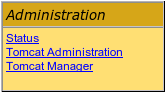
\includegraphics[scale=0.8]{graphics/tomcat_adminMenu}
   \caption{Tomcat \textit{Administration}-Men�}
   \label{img:tomcatadminmenu}
\end{figure}


Es �ffnet sich ein Fenster, in dem Benutzername und Kennwort des (unter Umst�nden soeben angelegten) Benutzers einzutragen sind. Auf der Manager-Seite ist nun unter \textit{Lokale WAR Datei zur Installation hochladen} das Archiv \textit{ATFrogs.war} �ber 
\includegraphics[scale=0.6]{graphics/button_durchsuchen.png} auszuw�hlen. Anschlie�end wird dieses mittels 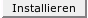
\includegraphics[scale=0.6]{graphics/button_installieren.png} hochgeladen und installiert (vgl. Abbildung \ref{img:tomcatmanagerinstall}).\

\begin{figure}[htb]
   \centering
   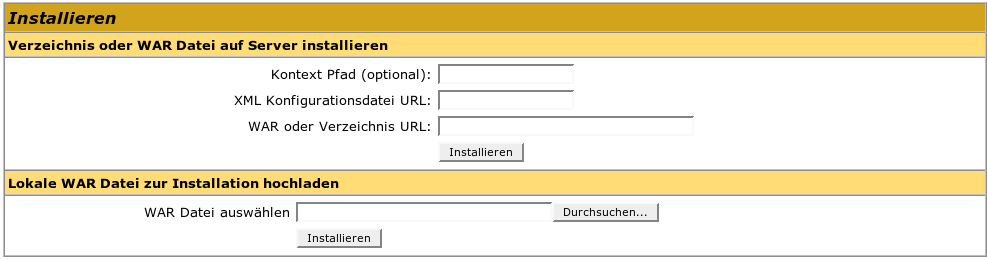
\includegraphics[width=\textwidth]{graphics/tomcat_managerinstall}
   \caption{Tomcat Manager Installationsdialog}
   \label{img:tomcatmanagerinstall}
\end{figure}

Wenn die Installation ohne Fehler abgelaufen ist, erscheint \ATFROGS, wie in Abbildung \ref{img:tomcatmanagercorrectinstalled} zu sehen, in der Liste der installierten Anwendungen.\

\begin{figure}[htb]
   \centering
   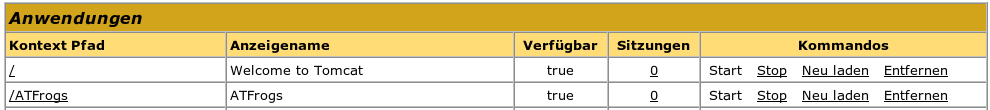
\includegraphics[width=\textwidth]{graphics/tomcat_managercorrectinstalled}
   \caption{Tomcat Manager Anwendungen}
   \label{img:tomcatmanagercorrectinstalled}
\end{figure}

\pagebreak

\subsection{Editieren der Konfigurationsdateien}\label{sect:install:konfigurationsdateien}
Nachdem die \ATFROGSnosp-Web-Applikation korrekt installiert wurde, muss sowohl die globale Konfigurationsdatei des Tomcat-Servers (\textit{server.xml}) als auch die Konfigurationsdatei der Web-Applikation (\textit{web.xml}) angepasst werden.\\
 
\NOTE{Die folgenden Schritte m�ssen im Kontext des Benutzers \textit{root} auf dem \OPENXCHANGE-Server durchgef�hrt werden.\\[2mm]
Vor dem �ndern einer Konfigurationsdatei sollte in jedem Fall eine Kopie dieser Datei angelegt werden, um den Vorgang r�ckg�ngig machen zu k�nnen.}\vspace*{5mm}

Im Anhang \ref{server.inc.xml} und \ref{web.inc.xml} finden sich die zu berarbeitenden Ausschnitte der Dateien \textit{server.xml} und \textit{web.xml} als Listings. Die im Folgenden angegebenen Zeilenangaben beziehen sich auf die Zeilenangaben innerhalb dieser Listings. Im Verzeichnnis parallel zu diesem Dokument finden sich die vollst�ndigen Dateien einer Musterkonfiguration anhand derer die eigenen Dateien angepasst werden k�nnen.

\subsubsection{Editieren der \textit{server.xml}}\label{sect:install:editserver.xml}
	In der Datei \textit{server.xml} im Ordner \textit{conf/} im Tomcat-Verzeichnis (zum Beispiel unter \textit{/usr/share/tomcat5}) werden globale Einstellungen f�r den Tomcat-Server definiert. Hier m�ssen Eintr�ge f�r die Authentifizierung der \ATFROGSnosp-Benutzer gegen den (auch von \OPENXCHANGEsp benutzten) LDAP-Server gemacht werden.\\
	
	Dazu muss innerhalb des existierenden \textbf{\texttt{Host}}-Tags f�r \texttt{localhost} ein \textbf{\texttt{Context}}-Tag eingef�gt werden (siehe Anhang \ref{server.inc.xml}).\\

	Die \texttt{connection}-Parameter (Zeilen 381 bis 383 des Listings in \ref{server.inc.xml}) m�ssen dabei f�r den zu benutzenden LDAP-Server angepasst werden. Au�erdem m�ssen die Parameter \texttt{userPattern} und \texttt{roleBase} (Zeilen 386 und 387) so angepasst werden, dass sie mit den Benutzern bzw. Gruppen �bereinstimmen, die \OPENXCHANGEsp im LDAP anlegt.\\

	\NOTE{Zu beachten ist, dass alle Benutzer, die \ATFROGS benutzen sollen, ihr Passwort mit dem Algorithmus verschl�sseln m�ssen, der innerhalb des Parameters \texttt{digest} (Zeile 391) angegeben ist.}

\pagebreak
	
\subsubsection{Editieren der \textit{web.xml}}\label{sect:install:editweb.xml}

	In der Datei \textit{web.xml} im Ordner \textit{webapps/ATFrogs/WEB-INF/web.xml} des Tomcat-Verzeichnisses k�nnen diverse Einstellungen f�r \ATFROGS vorgenommen werden. Eine Beispielkonfiguration f�r die wichtigsten Einstellungen befindet sich im Anhang \ref{web.inc.xml}. Zun�chst einmal m�ssen innerhalb des \textbf{\texttt{servlet}}-Tags f�r das Servlet \textit{ATFrogs} (definiert im Tag \textbf{\texttt{servlet-name}}) die folgenden Parameter (definiert im Tag \textbf{\texttt{init-param}}) eingestellt werden:
	
	
	\begin{description}
		\item [user:] %\
		An dieser Stelle muss ein g�ltiger \OPENXCHANGE-Benutzer eingetragen werden.\\
		
		\NOTE{Dieser Benutzer sollte eigens f�r diesen Zweck angelegt werden und muss Mitglied mindestens einer \OPENXCHANGE-Gruppe sein.}
		
		\item [pass:]%\
		An dieser Stelle muss das Passwort des unter \texttt{user} eingetragenen Benutzers angegeben werden.\footnote{Das Passwort muss im Klartext angegeben werden. Aus diesem Grund ist darauf zu achten, dass kein Benutzer neben dem Benutzer \textit{tomcat} Zugriff auf die \textit{web.xml} hat.}
		
		\item [servleturl:]%\
		 Damit \ATFROGS Daten der Groupware abfragen kann, muss dieser Parameter auf \texttt{http://localhost/servlet/webdav.groupuser} gesetzt werden (auch hier unter der Voraussetzung, dass sich \OPENXCHANGEsp auf demselben Server befindet).
		 
		\item [logfile:]%\
		 Dieser Parameter gibt an, in welchem Verzeichnis die Log-Dateien von \ATFROGS abgelegt werden sollen und spezifiziert deren Prefix.\\
		 
		\NOTE{Denkbar ist das Anlegen eines Verzeichnisses \textit{/var/log/ATFrogs/}. Zu beachten ist hierbei, dass der Benutzer \texttt{tomcat} Schreibrecht f�r dieses Verzeichnis hat (\texttt{chown -R tomcat /var/log/ATFrogs/ \&\& chmod -R 700 /var/log/ATFrogs/}).}
		
		\item [logLevel:]%\ 
		 Mit Hilfe dieses Parameters l�sst sich festlegen, welche Aktionen von \ATFROGS in den \ATFROGSnosp-Log-Dateien und der Log-Datei des Tomcat-Servers aufgezeichnet werden sollen. G�ltige Werte sind dabei \texttt{off}, \texttt{normal} und \texttt{debug}.
		 
		\item [defaultCategorie:]%\
		 Dieser Parameter bestimmt, welches \ATFROGSnosp-Modul nach dem Einloggen angezeigt wird. G�ltige Werte sind \texttt{groups}, \texttt{resources} und \texttt{user}.
		 
		\item [language:]%\
		 Hier wird die in \ATFROGS benutzte Sprache eingestellt. G�ltige Werte sind hier \texttt{de} f�r Deutsch und \texttt{en} f�r Englisch.
	\end{description}
	
	\pagebreak
	
	In den weiteren \texttt{servlet}-Tags m�ssen gegebenenfalls die Pfade zu den Skripten, die von \OPENXCHANGEsp mitgeliefert werden, angepasst werden. Au�erdem sollte das Skript \texttt{resetuserpasswd}\footnote{Das Skript befindet sich im Verzeichnis \textit{build/sbin/} des extrahierten \ATFROGSnosp-Archivs.}, zum Zur�cksetzen von Benutzer-Passw�rtern, in das gleiche Verzeichnis kopiert werden, in dem sich auch die Skripte der \OPENXCHANGE-Installation befinden. Innerhalb des \textbf{\texttt{servlet}}-Tags f�r das Servlet \texttt{ATFrogs.user} l�sst sich �ber den Parameter \texttt{resetpassword} das Passwort angeben, das nach einem Zur�cksetzen G�ltigkeit hat.\\

\NOTE{Zu beachten ist, dass alle Skripte f�r den Benutzer \textit{tomcat} ausf�hrbar sein m�ssen.\\ Abschlie�end muss der Tomcat-Server neu gestartet werden, damit die �nderungen wirksam werden.}\vspace*{5mm}

	
Um einer anderen Gruppe als der Gruppe \textit{ATFrogsUsers} Zugriff zu den \ATFROGSnosp-Modulen zu gew�hren, ist der Wert des Parameters \texttt{role-name} innerhalb der \texttt{\textbf{security-constraint}}-Tags abzu�ndern (vgl. Zeile 22 des folgenden Listings). Zu beachten ist, dass diese �nderung in allen entsprechenden Tags innerhalb der \textit{web.xml} anzupassen ist.\\

\begin{small}
\lstset{numbers=left, numberstyle=\tiny, stepnumber=2, numbersep=5pt, language=xml}
\begin{lstlisting}[caption=Ausschnitt server.xml, captionpos=b, frame=single, breaklines=true, firstnumber=12, numberfirstline=false]
<security-constraint>
<web-resource-collection>
	<web-resource-name>Protected Area</web-resource-name>
	<!-- Define the context-relative URL(s) to be protected -->
	<!-- All resources protected unless otherwise
             listed in previous security-constraints -->
	<url-pattern>/ATFrogs</url-pattern>
</web-resource-collection>
<auth-constraint>
	<!-- Anyone with one of the listed roles may access this area -->
	<role-name>ATFrogsUsers</role-name>
</auth-constraint>
</security-constraint>
\end{lstlisting}
\end{small}

\pagebreak

\subsection{Anpassen der \OPENXCHANGE-\ Skripte}
Damit die \OPENXCHANGE-Skripte mittels \ATFROGS ausgef�hrt werden k�nnen, muss die Konfigurationsdatei \textit{admintools.conf}\footnote{Ab der \OPENXCHANGE-Version 0.8.0-4 befindet sich diese Datei in dem Verzeichnis \textit{/etc/ox}.} f�r die Skripte angepasst werden (dieser Schritt muss im Kontext des Benutzers \textit{root} ausgef�hrt werden). Angenommen ein Verzeichnis \textit{/var/ox/tmp} wurde angelegt, so muss der Pfad f�r die tempor�ren Dateien wie folgt ge�ndert werden:
\begin{verbatim}
...
# TEMPORARY FILE
TMPDIF="/var/ox/tmp/temporary_ldap_scripts.ldif"
...
\end{verbatim}

\NOTE{Dabei ist zu beachten, dass die Datei \textit{admintools.conf} f�r den Benutzer \textit{tomcat} lesbar ist und dass die unter \texttt{TMPDIF} angegebene Datei von ihm geschrieben werden kann.}

\subsection{Einrichten einer Gruppe f�r authorisierte Benutzer}\label{sect:install:gruppeeinrichten}
Um Groupware-Nutzern die Benutzung von \ATFROGS zu erlauben, m�ssen diese als Mitglied der \ATFROGSnosp-Administratoren-Gruppe, hier \textit{ATFrogsUsers}, hinzugef�gt werden (dieser Schritt muss im Kontext des Benutzers \textit{root} ausgef�hrt werden). Falls diese Gruppe noch nicht existiert, so muss diese wie folgt erstellt werden:
\begin{verbatim}
addgroup_ox --group=ATFrogsUsers
\end{verbatim}
Anschlie�end kann der, in der \textit{web.xml} angelegte, Benutzer mit folgendem Kommando der Gruppe \textit{ATFrogsUsers} hinzugef�gt werden:
\begin{verbatim}
addusertogroup --user=benutzerID --group=ATFrogsUsers
\end{verbatim}
Nachdem mindestens ein Benutzer Mitglied der Gruppe \textit{ATFrogsUsers} ist, kann dieser �ber die Gruppenverwaltung weitere Mitglieder zu der Gruppe \textit{ATFrogsUsers} hinzuf�gen (siehe Abschnitt \ref{sect:groupadministration}).

\subsection{Erster Zugriff auf ATFrogs}\label{sect:install:firstAccess}
Nachdem \ATFROGS installiert und konfiguriert wurde und Benutzer f�r den Zugriff authorisiert wurden, kann die Anwendung mit einem Internetzugangsprogramm unter der Adresse \texttt{http://[myOXServer]:8080/ATFrogs} erreicht werden (siehe Abbildung \ref{img:adresslocator}). 

\begin{figure}[htb]
   \centering
   
\includegraphics[width=\textwidth]{graphics/adress_locator}
   \caption{Aufruf von \ATFROGS}
   \label{img:adresslocator}
\end{figure}

\pagebreak

Um \ATFROGS unter der Adresse \texttt{http://[myOXServer]/ATFrogs} erreichen zu k�nnen, ist die Datei \textit{/etc/httpd/conf/workers2.properties} um den folgenden Eintrag zu erweitern:
\begin{verbatim}
[uri:/ATFrogs/*]
worker=ajp13:localhost:8009
\end{verbatim}
   
\section{Anmelden und Navigieren}

\subsection{Anmeldebildschirm}

Ist die Installation gem�� Abschnitt \ref{sect:install} erfolgreich abgeschlossen, erscheint nach Aufruf der entsprechenden Adresse im Internetzugangsprogramm der \ATFROGSnosp-Anmeldebildschirm wie in Abbildung \ref{img:login} dargestellt.\\

\begin{figure}[htp]
   \centering
   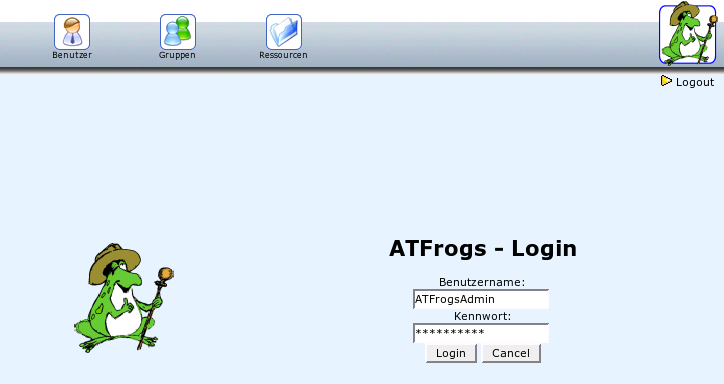
\includegraphics[width=\textwidth]{graphics/login}
   \caption{\ATFROGSnosp-Anmeldebildschirm}
   \label{img:login}
\end{figure}

Berechtigte Nutzer k�nnen sich nun an der Administrationsoberfl�che mit ihrem Benutzernamen und Kennwort anmelden. Ist die Anmeldung erfolgreich, gelangt man in die Ansicht einer der drei Module -- Benutzer, Gruppen oder Ressourcen (vgl. Abschnitt \ref{sect:install:editweb.xml}). Ist die Kombination von Benutzername und Kennwort falsch, so erscheint das Fenster erneut und die Eingabe kann korrigiert werden. \\

\subsection{Navigieren zwischen den Modulen}
Mit Hilfe der in Abbildung \ref{img:top_navigation} dargestellten Navigationsleiste, die sich in der Kopfzeile jedes Bildschirms befindet, l�sst sich bequem zwischen den drei \ATFROGSnosp-Modulen wechseln.

\begin{figure}[htp]
   \centering
   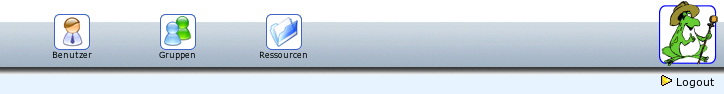
\includegraphics[width=\textwidth]{graphics/top_navigation}
   \caption{Navigationsleiste}
   \label{img:top_navigation}
\end{figure} 

\pagebreak
Die Navigationsleiste enth�lt die Symbole zum Zugriff auf die einzelnen \ATFROGSnosp-Module:


\begin{description}
\item[
\includegraphics{graphics/userlogo.png} Benutzeradministration]\

Durch einen Klick auf das Icon gelangt man in das Modul zur Benutzeradministration. Die Funktionen dieses Moduls werden in Kapitel \ref{sect:useradministration} dargestellt.
\item[
\includegraphics{graphics/grouplogo.png} Gruppenadministration]\

Durch einen Klick auf das Icon gelangt man in das Modul zur Gruppenadministration. Die Funktionen dieses Moduls werden in Kapitel \ref{sect:groupadministration} dargestellt.
\item[
\includegraphics{graphics/resourcelogo.png} Ressourcenadministration]\

Durch einen Klick auf das Icon gelangt man in das Modul zur Ressourcenadmi- nistration. Die Funktionen dieses Moduls werden in Kapitel \ref{sect:resourceadministration} dargestellt.
\end{description} \

Durch einen Klick auf 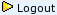
\includegraphics[scale=0.8]{graphics/logout.png} wird die aktuelle \ATFROGSnosp-Sitzung beendet. Wird diese Schaltfl�che gew�hlt, hat sich der Benutzer abgemeldet. Eine erneute Anmeldung vor der n�chsten Nutzung ist n�tig.\\

\NOTE{
Um unbefugte Zugriffe zu verhindern, sollte eine \ATFROGSnosp-Sitzung stets durch einen Klick auf 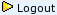
\includegraphics[scale=0.8]{graphics/logout.png} beendet werden!
}

\subsection{Einsehen der Konsolenausgabe}

Nach dem Durchf�hren einer Operation, die durch Ausf�hren eines der \OPENXCHANGE-Administrationsskripte realisiert wird, wird deren Konsolenausgabe in dem in Abbildung \ref{img:consoleOut} zu sehenden Textfeld unterhalb der Seite eingeblendet. 


\begin{figure}[htp]
   \centering
   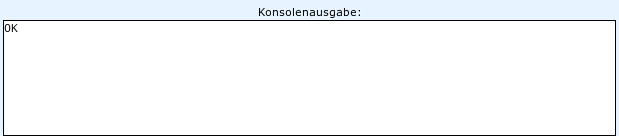
\includegraphics[width=\textwidth]{graphics/console_out}
   \caption{Anzeige der Konsolenausgabe}
   \label{img:consoleOut}
\end{figure} 





\section{Benutzeradministration}\label{sect:useradministration}

Durch einen Klick auf das in Abbildung \ref{img:iconUsers} dargestellte Symbol, das sich in der Navigationsleiste oberhalb jeder Seite findet, gelangt man in das \ATFROGSnosp-Modul zur Benutzeradministration. In diesem Modul lassen sich bestehende Benutzer einsehen und l�schen. Au�erdem kann das Passwort eines Benutzers auf das in der Konfigurationsdatei \texttt{web.xml} definierte Standardpasswort (siehe Abschnitt \ref{sect:install:konfigurationsdateien}) zur�ckgesetzt werden.

\begin{figure}[htp]
   \centering
   
\includegraphics[scale=1]{graphics/userlogo.png}
   \caption{Icon des \ATFROGSnosp-Moduls zur Benutzeradministration}
   \label{img:iconUsers}
\end{figure}

\subsection{Auswahl eines Benutzers}\label{sect:useradministration:auswahlbenutzer}
�ber das mit {\small{\texttt{Benutzername:}}} beschriftete Eingabefeld ist eine Suche nach Benutzern aus der Menge der \OPENXCHANGE-Benutzer m�glich. Hierzu muss ein Suchmuster in das Eingabefeld eingetragen werden. Das Sternchen (\texttt{*}) kann als Platzhalter f�r beliebig lange Zeichenfolgen genutzt werden und darf innerhalb des Suchmusters beliebig oft auftreten.\footnote{In Abbildung \ref{img:user_overview} erscheint als Ergebnis der Suchanfrage \texttt{*ueller*} der Name Hans Mueller -- in der Annahme, dass dessen Benutzername \textit{Mueller} ist. Die Anfragen \texttt{Mueller} und \texttt{*ueller} w�rden zu demselben Ergebnis f�hren. W�rde ein Benutzer mit dem Benutzernamen \textit{Muellermeyer} existieren, so w�rde auch dieser in der Ergebnisliste der Anfrage \texttt{*ueller*} erscheinen, in der Ergebnisliste der beiden anderen Anfragen hingegen nicht. Zu beachten ist, dass das Sternchen (\texttt{*}) auch als Platzhalter f�r eine leere Zeichenfolge stehen kann.} Die Suche wird durch einen Klick auf 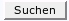
\includegraphics[scale=0.6]{graphics/button_search2.png} gestartet. Das Suchergebnis wird anschlie�end in der Liste unterhalb des Eingabefeldes dargestellt (siehe Abbildung \ref{img:user_overview}).\\

\begin{figure}[htp]
   \centering
   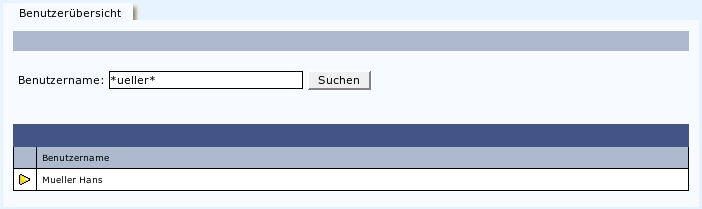
\includegraphics[width=\textwidth]{graphics/user_overview}
   \caption{Suche nach einem Benutzer}
   \label{img:user_overview}
\end{figure}

\NOTE{Durchsucht werden die Benutzernamen (UIDs) der Benutzer. Andere Felder wie Vorname oder Nachname werden nicht durchsucht!}\\[1cm]

\pagebreak

Nach einer erfolgreichen Suche ist es m�glich, sich die Details zu einem Benutzer anzusehen. Dazu muss auf den Benutzernamen in der Liste unterhalb des Eingabefeldes geklickt werden. Anschlie�end erscheint die Detailansicht zu dem Benutzer (siehe Abbildung \ref{img:user_details}).
\begin{figure}[htp]
   \centering
   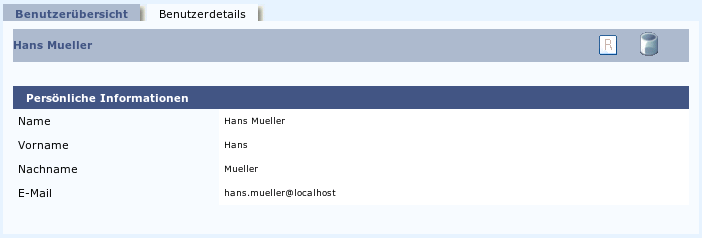
\includegraphics[width=\textwidth]{graphics/user_details}
   \caption{Detailansicht eines Benutzers}
   \label{img:user_details}
\end{figure}

\subsection{Zur�cksetzen des Passworts}\label{sect:useradministration:resetuserpwd}
Vorausgesetzt das Skript \textit{resetuserpwd} ist installiert (siehe Abschnitt \ref{sect:install:editweb.xml}), so kann das Passwort f�r einen Benutzer zur�ckgesetzt werden. Daf�r muss zun�chst einmal der entsprechende Benutzer gesucht und ausgew�hlt werden (siehe Abschnitt \ref{sect:useradministration:auswahlbenutzer}).\\

In der Detailansicht kann nun durch einen Klick auf 
\includegraphics[scale=0.6]{graphics/icon_reset.png} das Passwort des zuvor ausgew�hlten Benutzers zur�ckgesetzt werden. Nachdem der Wunsch best�tigt wurde, ist die Operation durchgef�hrt.

\subsection{L�schen eines Benutzers}
Um einen \OPENXCHANGE-Benutzer zu l�schen, muss dieser zun�chst einmal gesucht und ausgew�hlt werden (siehe Abschnitt \ref{sect:useradministration:auswahlbenutzer}).\\

In der Detailansicht kann der Benutzer durch einen Klick auf \ICON{graphics/icon_trash.png} gel�scht werden. Nachdem der Wunsch best�tigt wurde, ist der Benutzer endg�ltig gel�scht.\

\section{Gruppenadministration}\label{sect:groupadministration}

Durch einen Klick auf das in Abbildung \ref{img:iconGroups} dargestellte Symbol, das sich in der Navigationsleiste oberhalb jeder Seite findet, gelangt man in das \ATFROGSnosp-Modul zur Grup- penadministration. In diesem Modul lassen sich bestehende Gruppen einsehen und l�schen. Benutzer k�nnen zu den Gruppen hinzugef�gt oder aus diesen entfernt werden. Neue Gruppen k�nnen erstellt werden.

\begin{figure}[htp]
   \centering
   
\includegraphics[scale=1]{graphics/grouplogo.png}
   \caption{Icon des \ATFROGSnosp-Moduls zur Gruppenadministration}
   \label{img:iconGroups}
\end{figure}

\subsection{�bersicht aller Gruppen}\label{sect:groupOverview}

Nach Auswahl des Moduls gelangt man in die in Abbildung \ref{img:group_overview} dargestellte, alphabetisch geordnete �bersicht aller existierender Gruppen. Durch einen Klick auf den Namen einer Gruppe bzw. auf das nebenstehende Symbol 
\includegraphics[scale=0.7]{graphics/arrow_right} gelangt man in deren Detailansicht, die im folgenden Abschnitt \ref{sect:groupDetails} behandelt wird.

\begin{figure}[htp]
   \centering
   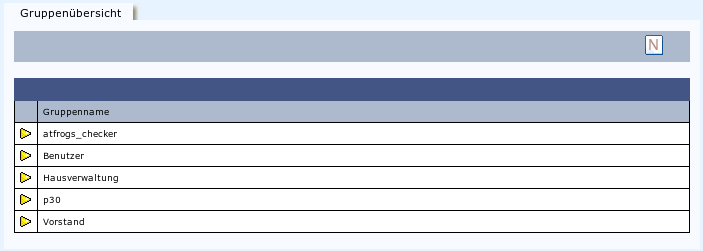
\includegraphics[width=\textwidth]{graphics/group_overview}
   \caption{�bersicht aller Gruppen}
   \label{img:group_overview}
\end{figure}

\subsection{Detailansicht einer Gruppe}\label{sect:groupDetails}

Nach Auswahl einer Gruppe in der im Abschnitt \ref{sect:groupOverview} dargestellten Gruppen�bersicht gelangt man in deren Detailansicht. Abbildung \ref{img:group_details} zeigt ein Beispiel daf�r. In der mit {\small\texttt{Mitglieder:}} beschrifteten Liste werden die Benutzer angezeigt, die der Gruppe zugeordnet sind.

\begin{figure}[htp]
   \centering
   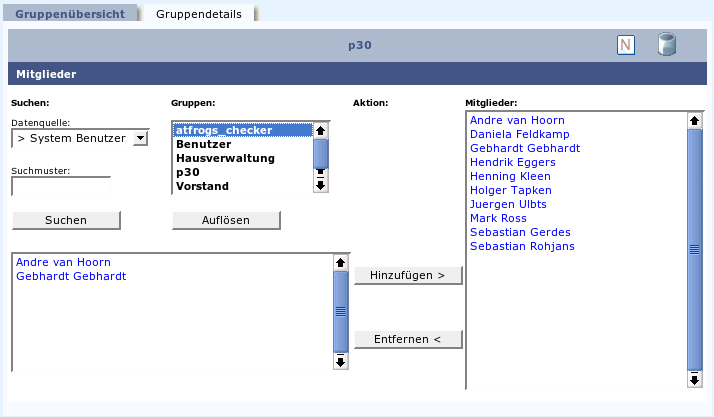
\includegraphics[width=\textwidth]{graphics/group_details}
   \caption{Detailansicht einer Gruppe}
   \label{img:group_details}
\end{figure}

\subsubsection{Hinzuf�gen und Entfernen von Benutzern}
   
Mit Hilfe der Schaltfl�chen 
\includegraphics[scale=0.6]{graphics/button_elementAdd.png} und

\includegraphics[scale=0.6]{graphics/button_elementRemove.png} lassen sich Benutzer zu der Gruppe hinzuf�gen bzw. aus dieser entfernen. \\

\paragraph{Entfernen von Benutzern}\

Sollen Benutzer aus der aktuell gew�hlten Gruppe entfernt werden, so m�ssen diese zun�chst in der Liste der Mitglieder selektiert werden. Einzelne Benutzer lassen sich durch einen einfachen Klick selektieren. Mehrere Benutzer lassen sich durch Halten der {\small{\texttt{Strg}}}-Taste w�hrend des gesamten Selektionsvorgangs ausw�hlen. Durch einen Klick auf 
\includegraphics[scale=0.6]{graphics/button_elementRemove.png} werden die selektierten Benutzer ohne weitere Nachfrage aus der Gruppe entfernt.

\paragraph{Hinzuf�gen von Benutzern}\

Damit Benutzer zur Gruppe hinzugef�gt werden k�nnen, m�ssen in Frage kommende Benutzer in der Liste im Dialog links unten (siehe Abbildung \ref{img:group_details}) angezeigt werden. \ATFROGS bietet hier die beiden aus \OPENXCHANGEsp bekannten Varianten:

\begin{itemize}
\item \textbf{Suche nach Benutzern}\

�ber das mit {\small{\texttt{Suchmuster:}}} beschriftete Eingabefeld ist eine Suche nach Benutzern aus der Menge der \OPENXCHANGE-Benutzer m�glich. Hierzu muss ein Suchmuster in das Eingabefeld eingetragen werden. Das Sternchen (\texttt{*}) kann als Platzhalter f�r beliebig lange Zeichenfolgen genutzt werden und darf innerhalb des Suchmusters beliebig oft auftreten.\footnote{Beispiele f�r die Suche mittels Suchmustern finden sich in Abschnitt \ref{sect:useradministration:auswahlbenutzer}.} Die Suche wird durch einen Klick auf 
\includegraphics[scale=0.6]{graphics/button_search.png} gestartet. Das Suchergebnis wird anschlie�end in der Liste der Suchergebnisse angezeigt.\\

\NOTE{
Durchsucht werden die Benutzernamen (UIDs) der Benutzer. Andere Felder wie Vorname oder Nachname werden nicht durchsucht!
}

\item \textbf{Aufl�sen von Gruppen}\

Neben der Suche nach Benutzern ist das Aufl�sen von Gruppen m�glich. Die Gruppen m�ssen hierzu in der Liste unterhalb von {\small{\texttt{Gruppen:}}} selektiert werden (Mehrfachauswahl mit der {\small{\texttt{Strg}}}-Taste). Ein Klick auf 
\includegraphics[scale=0.6]{graphics/button_extract.png} l�st das Aufl�sen der Gruppen aus. Aus Abbildung \ref{img:group_details} ist das Ergebnis einer solchen Operation, angewendet auf die Gruppe \textit{atfrogs\_checker}, ersichtlich.
\end{itemize} 

Aus dem Ergebnis des Suchvorgangs oder des Aufl�sens von Gruppen lassen sich nun hinzuzuf�gende Benutzer ausw�hlen (Mehrfachauswahl mit der {\small{\texttt{Strg}}}-Taste). Die Operation wird durch einen Klick auf 
\includegraphics[scale=0.6]{graphics/button_elementAdd.png} durchgef�hrt. Die Benutzer erscheinen nun in der Liste der Mitglieder.

\subsubsection{L�schen einer Gruppe}

�ber den in Abbildung \ref{img:group_details} dargestellten Dialog l�sst sich die gew�hlte Gruppe l�schen. Hierzu ist ein Klick auf das Symbol \ICON{graphics/item_delete.png} notwendig. Es folgt eine Sicherheitsabfrage, um ein versehentliches L�schen von Gruppen zu verhindern. Wird das L�schen best�tigt, gelangt man zur�ck zur �bersicht aller Gruppen. Andernfalls kehrt man zur�ck in den aus Abbildung \ref{img:group_details} bekannten Dialog.

\subsection{Anlegen neuer Gruppen}\label{sect:group:new}

Durch einen Klick auf das Symbol \ICON{graphics/item_new.png} (existiert sowohl in der Gruppen�bersicht als auch in der Detailansicht einer Gruppe) gelangt man in den Dialog zum Anlegen einer neuen Gruppe (siehe Abbildung \ref{img:group_new}). In das Textfeld kann der gew�nschte Name f�r die neue Gruppe eingetragen werden.\footnote{Zu beachten ist, dass Leerzeichen innerhalb eines Namens nicht zul�ssig sind. Umlaute oder Sonderzeichen sollten ebenfalls vermieden werden.} Durch einen Klick auf 
\includegraphics[scale=0.6]{graphics/button_doNew.png} wird die Gruppe angelegt. War dieser Vorgang erfolgreich, gelangt man in die Detailansicht der neuen Gruppe. Im Fehlerfall besteht die M�glichkeit der Korrektur der get�tigten Eingabe. Durch einen Klick auf 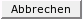
\includegraphics[scale=0.6]{graphics/button_doCancel.png} wird der Vorgang abgebrochen und man gelangt zur �bersicht aller bestehenden Gruppen.

\begin{figure}[htp]
   \centering
   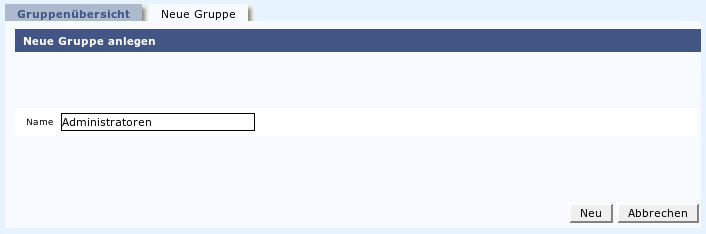
\includegraphics[width=\textwidth]{graphics/group_new}
   \caption{Anlegen einer neuen Gruppe}
   \label{img:group_new}
\end{figure}



\section{Ressourcenadministration}\label{sect:resourceadministration} 

Durch einen Klick auf das in Abbildung \ref{img:iconResources} dargestellte Symbol, das sich in der Navigationsleiste oberhalb jeder Seite findet, gelangt man in das \ATFROGSnosp-Modul zur Ressourcenadministration. In diesem Modul lassen sich bestehende Ressourcen und Ressourcengruppen einsehen und l�schen. Ressourcen k�nnen zu den Ressourcengruppen hinzugef�gt oder aus diesen entfernt werden. Neue Ressourcen und Ressourcengruppen k�nnen erstellt werden.

\begin{figure}[htp]
   \centering
   
\includegraphics[scale=1]{graphics/resourcelogo.png}
   \caption{Icon des \ATFROGSnosp-Moduls zur Ressourcenadministration}
   \label{img:iconResources}
\end{figure}

\subsection{�bersicht aller Ressourcengruppen}\label{sect:resgrpOverview}
Nach Auswahl des Moduls gelangt man in die in Abbildung \ref{img:resgrp_overview} dargestellte, alphabetisch geordnete �bersicht aller existierender Ressourcengruppen. Durch einen Klick auf den Namen einer Gruppe bzw. auf das nebenstehende Symbol 
\includegraphics[scale=0.7]{graphics/arrow_right} gelangt man in deren Detailansicht, die im folgenden Abschnitt \ref{sect:resgroupDetails} behandelt wird.

\begin{figure}[htp]
   \centering
   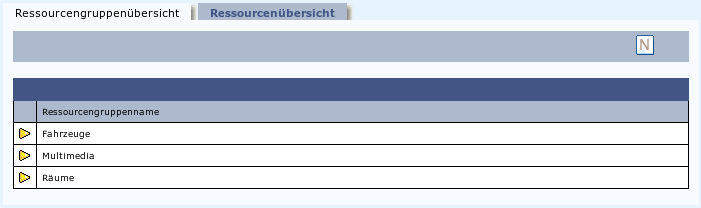
\includegraphics[width=\textwidth]{graphics/resgrp_overview}
   \caption{�bersicht aller Ressourcengruppen}
   \label{img:resgrp_overview}
\end{figure}

\subsection{Detailansicht einer Ressourcengruppe}\label{sect:resgroupDetails}

Nach Auswahl einer Ressourcengruppe in der im Abschnitt \ref{sect:resgrpOverview} dargestellten Gruppen�bersicht gelangt man in deren Detailansicht. Abbildung \ref{img:resgrp_details} zeigt ein Beispiel daf�r. In der mit {\small\texttt{Ressourcen:}} beschrifteten Liste werden die Ressourcen angezeigt, die der Gruppe zugeordnet sind.
\begin{figure}[htp]
   \centering
   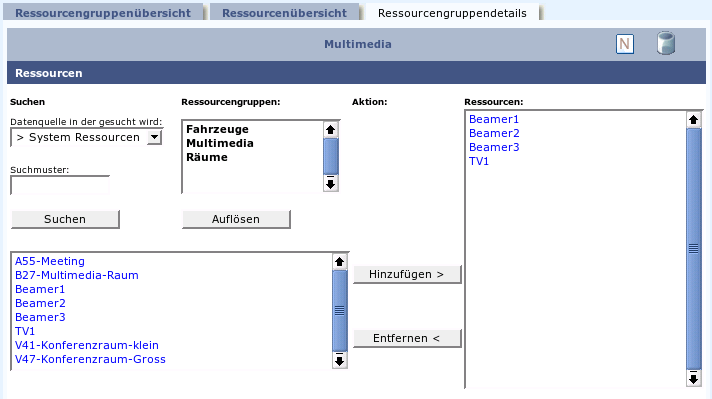
\includegraphics[width=\textwidth]{graphics/resgrp_details}
   \caption{Detailansicht einer Ressourcengruppe}
   \label{img:resgrp_details}
\end{figure}

\subsubsection{Hinzuf�gen und Entfernen von Ressourcen}
   
Mit Hilfe der Schaltfl�chen 
\includegraphics[scale=0.6]{graphics/button_elementAdd.png} und

\includegraphics[scale=0.6]{graphics/button_elementRemove.png} lassen sich Ressourcen zu der Ressourcengruppe hinzuf�gen bzw. aus dieser entfernen. \\
   
\paragraph{Entfernen von Ressourcen}\

Sollen Ressourcen aus der aktuell gew�hlten Ressourcengruppe entfernt werden, so m�ssen diese zun�chst in der Liste der der Gruppe zugeordneten Ressourcen selektiert werden. Einzelne Ressourcen lassen sich durch einen einfachen Klick selektieren. Mehrere Ressourcen lassen sich durch Halten der {\small{\texttt{Strg}}}-Taste w�hrend des gesamten Selektionsvorgangs ausw�hlen. Durch einen Klick auf 
\includegraphics[scale=0.6]{graphics/button_elementRemove.png} werden die selektierten Ressourcen ohne weitere Nachfrage aus der Ressourcengruppe entfernt.

\paragraph{Hinzuf�gen von Ressourcen}\

Damit Ressourcen zur Gruppe hinzugef�gt werden k�nnen, m�ssen in Frage kommende Elemente in der Liste im Dialog links unten (siehe Abbildung \ref{img:group_details}) angezeigt werden. \ATFROGS bietet auch an dieser Stelle die beiden aus \OPENXCHANGEsp bekannten Varianten:

\begin{itemize}
\item \textbf{Suche nach Ressourcen}\

�ber das mit {\small{\texttt{Suchmuster:}}} beschriftete Eingabefeld ist eine Suche nach Ressourcen aus der Menge der \OPENXCHANGE-Ressourcen m�glich. Hierzu muss ein Suchmuster in das Eingabefeld eingetragen werden. Das Sternchen (\texttt{*}) kann als Platzhalter f�r beliebig lange Zeichenfolgen genutzt werden und darf innerhalb des Suchmusters beliebig oft auftreten.\footnote{Beispiele f�r die Suche mittels Suchmustern finden sich in Abschnitt \ref{sect:useradministration:auswahlbenutzer}.} Die Suche wird durch einen Klick auf 
\includegraphics[scale=0.6]{graphics/button_search.png} gestartet. Das Suchergebnis wird anschlie�end in der Liste der Suchergebnisse angezeigt. Aus Abbildung \ref{img:resgrp_details} ist das Ergebnis einer solchen Operation -- mit dem Suchmuster \glqq \texttt{*}\grqq\ -- ersichtlich.\\

\pagebreak

\item \textbf{Aufl�sen von Ressourcengruppen}\

Neben der Suche nach Ressourcen ist das Aufl�sen von Ressourcengruppen m�glich. Die Gruppen m�ssen hierzu in der Liste unterhalb von {\small{\texttt{Ressourcengruppen:}}} selektiert werden (Mehrfachauswahl mit der {\small{\texttt{Strg}}}-Taste). Ein Klick auf 
\includegraphics[scale=0.6]{graphics/button_extract.png} l�st das Aufl�sen der Gruppen aus. 
\end{itemize} 

Aus dem Ergebnis des Suchvorgangs oder des Aufl�sens von Gruppen lassen sich nun hinzuzuf�gende Ressourcen ausw�hlen (Mehrfachauswahl mit der {\small{\texttt{Strg}}}-Taste). Das Hinzuf�gen wird durch einen Klick auf 
\includegraphics[scale=0.6]{graphics/button_elementAdd.png} durchgef�hrt. 

\subsubsection{L�schen einer Ressourcengruppe}

�ber den in Abbildung \ref{img:resgrp_details} dargestellten Dialog l�sst sich die gew�hlte Ressourcengruppe l�schen. Hierzu ist ein Klick auf das Symbol \ICON{graphics/item_delete.png} notwendig. Es folgt eine Sicherheitsabfrage, um ein versehentliches L�schen von Ressourcengruppen zu verhindern. Wird das L�schen best�tigt, gelangt man zur�ck zur �bersicht aller Ressourcengruppen. Andernfalls kehrt man zur�ck in den aus Abbildung \ref{img:resgrp_details} bekannten Dialog.

\subsection{�bersicht aller Ressourcen}\label{sect:resOverview}
Durch einen Klick auf die Titelzeile der mit 
\includegraphics[scale=0.7]{graphics/res_tab_resoverview.png} beschrifteten Karteikarte gelangt man in die alphabetisch geordnete �bersicht aller existierender Ressourcen, die in Abbildung \ref{img:res_overview} dargestellt ist. 

\begin{figure}[htp]
   \centering
   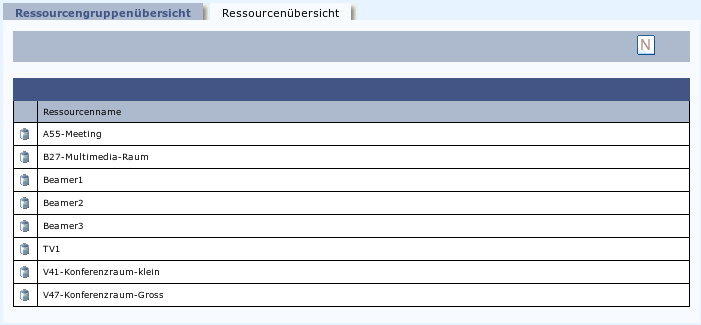
\includegraphics[width=\textwidth]{graphics/res_overview}
   \caption{�bersicht aller Ressourcen}
   \label{img:res_overview}
\end{figure}

\subsubsection{L�schen einer Ressource}

�ber den in Abbildung \ref{img:res_overview} dargestellten Dialog lassen sich einzelne Ressourcen l�schen. Hierzu ist ein Klick auf das Symbol %
\includegraphics[scale=0.7]{graphics/delete_res.png}
 \ICON{graphics/item_delete.png} links neben der zu l�schenden Ressource notwendig. Es folgt eine Sicherheitsabfrage, um ein versehentliches L�schen zu verhindern.

\subsection{Anlegen neuer Ressourcen oder Ressourcengruppen}

Durch einen Klick auf das Symbol \ICON{graphics/item_new.png} gelangt man in den kombinierten Dialog zum Anlegen einer neuen Ressource oder Ressourcengruppe (siehe Abbildung \ref{img:res_new}). In das Textfeld kann der gew�nschte Name eingetragen werden.\footnote{Wie im Abschnitt \ref{sect:group:new} im Zusammenhang mit der Vergabe von Namen f�r neue Gruppen erw�hnt, ist auch hier zu beachten, dass Leerzeichen innerhalb eines Namens nicht zul�ssig sind. Umlaute oder Sonderzeichen sollten ebenfalls vermieden werden.} Unterhalb des Textfeldes muss die Auswahl des neu anzulegenden Elementtyps vorgenommen werden. Durch einen Klick auf 
\includegraphics[scale=0.6]{graphics/button_doNew.png} wird dieses angelegt. War der Vorgang erfolgreich, gelangt man -- abh�ngig davon, ob eine neue Ressource oder eine neue Ressourcengruppe angelegt wurde -- in die Detailansicht der neuen Ressourcengruppe oder zur �bersicht aller Ressourcen. Im Fehlerfall besteht die M�glichkeit der Korrektur der get�tigten Eingabe. Durch einen Klick auf 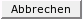
\includegraphics[scale=0.6]{graphics/button_doCancel.png} wird der Vorgang abgebrochen.

\begin{figure}[htp]
   \centering
   \includegraphics[width=\textwidth]{graphics/res_new}
   \caption{Anlegen einer neuen Ressource}
   \label{img:res_new}
\end{figure}



\section{Troubleshooting}\label{sect:troubleshooting}

Sollten w�hrend der Installation oder der Nutzung von \ATFROGS Probleme auftreten, sind die folgenden Schritte grunds�tzlich durchzuf�hren:

\begin{itemize}
\item Analysieren der Fehlermeldung innerhalb von \ATFROGS
\item Einsehen der \ATFROGSnosp-Log-Dateien
\item Einsehen der Tomcat-Log-Dateien
\end{itemize} 

\NOTE{Ist das Attribut \texttt{logLevel} in der \texttt{web.xml} auf \texttt{off}, so werden keine Meldungen in die \ATFROGSnosp-Log-Dateien geschrieben. Im Level \texttt{debug} ist der Umfang der geschriebenen Informationen am gr��ten (vgl. Abschnitt \ref{sect:install:editweb.xml}).}\vspace{5mm}

Im Folgenden werden h�ufig autretende Fehler und L�sungsans�tze aufgef�hrt.\


\subsection*{Kein Zugriff auf den Tomcat-Manager}
\textbf{Problembeschreibung:} �ber \url{http://[myOXServer]:8080}\ ist kein Zugriff auf den Tomcat-Manager m�glich.\\
\textbf{M�gliche L�sung: } �berpr�fen Sie die Einstellungen der Server-Firewall bez�glich des Ports 8080. Zumindest vom Server aus sollte ein Zugriff �ber \url{http://localhost:8080}\ m�glich sein. \\

\subsection*{Web-Applikation nicht im Tomcat-Manager}
\textbf{Problembeschreibung:} \ATFROGS erscheint nach der Installation der Web-Applikation durch den Tomcat-Manager nicht in dessen Liste der installierten Anwendungen.\\
\textbf{M�gliche L�sung: } Der Benutzer \textit{tomcat} verf�gt nicht �ber die entsprechenden Rechte im Ordner \textit{webapps} des Tomcat-Verzeichnisses. Mit \texttt{chown -R tomcat webapps/} sollte dies ge�ndert werden.\\

\subsection*{Anmeldung an \ATFROGS nicht m�glich}
\textbf{Problembeschreibung:} Die Login-Seite von \ATFROGS erscheint, jedoch ist das Anmelden nicht m�glich. \\
\textbf{M�gliche L�sung:} Der einfachste Fall ist, dass Benutzername oder Kennwort falsch sind. Ist dies nicht der Fall, wurde die Authentifikation in der \texttt{server.xml} m�glicherweise fehlerhaft eingestellt (vgl. Abschnitt \ref{sect:install:editserver.xml}). Weitere Informationen k�nnte die \texttt{localhost}-Log-Datei des Tomcat liefern. Stellen Sie au�erdem sicher, dass der Benutzer der Gruppe der \ATFROGSnosp-Administratoren zugeordnet ist. Sollte das Anmelden trotzdem nicht m�glich sein, so k�nnte das Kennwort des Benutzers m�glicherweise nicht mit dem in der \texttt{server.xml} angegebenen Mechanismus verschl�sselt sein. Loggen Sie sich dazu mit dem entsprechenden Benutzer in der Groupware ein und �ndern Sie den Verschl�sselungsmechanismus entsprechend.

\subsection*{Fehlermeldung nach dem Anmelden}
\textbf{Problembeschreibung:} Das Anmelden an \ATFROGS ist erfolgreich, jedoch wird statt eines \ATFROGSnosp-Moduls eine Meldung eines schwer wiegenden Fehlers angezeigt. \\
\textbf{M�gliche L�sung:} In diesem Fall sollten vor allem die Log-Datei des Tomcat eingesehen werden. M�glicherweise sind die in der \texttt{web.xml} eingetragenen Daten fehlerhaft (Benutzername oder Kennwort des dort eingetragenen Benutzers) oder der Benutzer ist in keiner \OPENXCHANGE-Gruppe. Stellen Sie au�erdem sicher, dass die \OPENXCHANGE-WebDAV-Schnittstelle korrekt funktioniert.\\

\subsection*{Logger kann nicht initialisiert werden}
\textbf{Problembeschreibung:} Das Anmelden an \ATFROGS ist erfolgreich, jedoch wird statt eines \ATFROGSnosp-Moduls die Meldung \textit{cannot initiate the logger} angezeigt. \\
\textbf{M�gliche L�sung:} Der Benutzer \textit{tomcat} verf�gt nicht �ber die entsprechenden Berechtigungen im Verzeichnis der \ATFROGSnosp-Log-Dateien oder ein solches Verzeichnis existiert nicht. �berpr�fen Sie die von Ihnen durchgef�hrten Schritte im Abschnitt \ref{sect:install:editweb.xml}\\


\appendix

\section{Anhang}\label{sect:anhang}

Die folgenden beiden Abschnitte \ref{server.inc.xml} und \ref{web.inc.xml} enthalten die Listings der beiden Konfigurationsdateien \textit{server.xml} und \textit{web.xml}, die gem�� Abschnitt \ref{sect:install:konfigurationsdateien} anzupassen sind. Vollst�ndige Musterdateien finden sich in dem Verzeichnis, in dem sich auch dieses Dokument innerhalb des Archivs \textit{atfrogs-<version>.tar.gz} befindet. 

\subsection{Ausschnitt \textit{server.xml}}\label{server.inc.xml}
Das folgende Listing enh�lt einen Ausschnitt aus der Konfigurationsdatei \textit{server.xml} mit beispielhaften Einstellungen f�r die Authentifizierung der \ATFROGSnosp-Benutzer gegen den (auch von \OPENXCHANGEsp benutzten) LDAP-Server.\\

\begin{small}
\lstset{numbers=left, numberstyle=\tiny, stepnumber=2, numbersep=5pt, language=xml}
\begin{lstlisting}[caption=Ausschnitt server.xml, captionpos=b, frame=single, breaklines=true, firstnumber=373, numberfirstline=false]
        <Logger className="org.apache.catalina.logger.FileLogger"
         directory="logs"  prefix="localhost_log." suffix=".txt"
         timestamp="true"/>

        <Context path="/ATFrogs" docBase="ATFrogs" debug="9" 
         reloadable="true" >
          <Realm className="org.apache.catalina.realm.JNDIRealm"
           debug="99"
           connectionName="cn=Manager,dc=YOUR-COMPANY,dc=de"
           connectionPassword="YOUR-PASSWORD"
           connectionURL="ldap://GROUPWARE.YOUR-COMPANY:389"
           userSearch="(uid={1})"
           userPassword="userPassword"
           userPattern="uid={0},ou=Users,ou=OxObjects,dc=your-company,dc=de"
           roleBase="ou=Groups,ou=OxObjects,dc=your-company,dc=de"
           roleName="cn"
           roleSearch="(memberUid={1})"
           roleSubtree="false"
           digest="SHA"/>
        </Context>

      </Host>

    </Engine>

  </Service>

</Server>
\end{lstlisting}
\end{small}

\pagebreak

\subsection{Ausschnitt \textit{web.xml}}\label{web.inc.xml}
Das folgende Listing enh�lt einen Ausschnitt aus der Konfigurationsdatei \textit{web.xml} mit den wichtigsten Einstellungen.\\

\begin{small}
\lstset{numbers=left, numberstyle=\tiny, stepnumber=2, numbersep=5pt, language=xml}
\begin{lstlisting}[caption=Ausschnitt web.xml, captionpos=b, frame=single, breaklines=true, firstnumber=80]
<servlet>
  <servlet-name>ATFrogs</servlet-name>
  <servlet-class>atfrogs.servlets.ATFrogsMainServlet</servlet-class>
  <init-param>
    <param-name>user</param-name>
    <param-value>mailadmin</param-value>
  </init-param>
  <init-param>
    <param-name>pass</param-name>
    <param-value>YOUR-PASSWORD</param-value>
  </init-param>
  <init-param>
    <param-name>servleturl</param-name>
    <param-value>http://localhost/servlet/webdav.groupuser</param-value>
  </init-param>
  <init-param>
    <!-- tomcat user must of write access to directory
         tip: create directory for these log files -->
    <param-name>logfile</param-name>
    <param-value>/var/log/ATFrogs/ATFrogs.log</param-value>
  </init-param>
  <init-param>
    <!-- To specify level of logging. Possible values are:
         off    - no logging
         normal - logging of user actions (default)
         debug  - additional messages for debugging
         Note: Also concerns output to catalina.out -->
    <param-name>logLevel</param-name>
    <param-value>debug</param-value>
  </init-param>	
  <init-param>
    <!-- categorie to show after login {groups | resources | user } -->
    <param-name>defaultCategorie</param-name>
    <param-value>groups</param-value>
  </init-param>	
  <init-param>
    <!-- language {en | de} -->
    <param-name>language</param-name>
    <param-value>de</param-value>
  </init-param>
</servlet>
\end{lstlisting}
\end{small}


%\newpage
%\section{Glossar}
%%%Allgeimeine Vorlage

%Artikel auf A4 Papier
\documentclass[12pt, a4paper]{article} 
 
\newcommand{\doctitle}
{ATFrogs - Handbuch}
 
%Deutsche Sprache, Silbentrennung, Grafikeinbindung
%Umlaute k{\"o}nnen direkt eingegeben werden
\usepackage[T1]{fontenc}
\usepackage[latin1]{inputenc}
\usepackage{ngerman}
\usepackage{times} 
\usepackage{mathptm}
\usepackage{fancyhdr}
\usepackage{makeidx}
\usepackage{longtable}

\usepackage{listings}

%%Erzwingt Ausgabe von Glossar- und Index-Dateien: anfdef.idx und anfdef.glo
\makeindex
\makeglossary
\renewcommand{\indexname}{}




%%Layout der Kopfzeile.
%\pagestyle{fancy} 
%\fancyhead[R]{\thepage}
%\fancyfoot[C]{}

\title{\doctitle}

%%Wenn pdflatex(f{\"u}r pdf-Dateien) verwendet wird, dann diese Zeile Verwenden
\usepackage[pdftex]{graphicx}
\usepackage{times}

\usepackage{textcomp} % u.a. TM-Zeichen
\usepackage{url}

\tolerance=10000 % Toleranz beim Trennen
% Disable single lines at the start of a paragraph (Schusterjungen)
\clubpenalty = 10000
%
% Disable single lines at the end of a paragraph (Hurenkinder)
\widowpenalty = 10000 \displaywidowpenalty = 10000

\newcommand{\TODO}[1]{ $\star \star \star$ \textbf{ TODO:  #1 }  $\star \star \star$}


\newcommand{\ICON} [1] { \includegraphics[scale=0.5] {#1} }
\newcommand{\ATFROGS}{\textit{ATFrogs}\ }
\newcommand{\ATFROGSnosp}{\textit{ATFrogs}}
\newcommand{\OPENXCHANGEsp}{\textit{Open-XChange}\texttrademark\ }
\newcommand{\OPENXCHANGE}{\textit{Open-XChange}\texttrademark}

\usepackage{color}
\newcommand{\NOTE}[1]{
    \hspace*{1cm}
    \fcolorbox{white}{red}{\fcolorbox{red}{white}{\parbox{0.8\textwidth}{
    	\textcolor{red}{{\sffamily \small \textbf{Hinweis:}}}\\
    	{\sffamily \textit{#1}}
    \hspace*{1cm}
    }}}
}

\usepackage[top=2.5cm, bottom=2.5cm, left=3.5cm, right=2.5cm]{geometry}


%%Layout der Kopfzeile.

\pagestyle{fancy}

\fancyhead[R]{\thepage}

\fancyfoot[C]{\ATFROGS Handbuch - August 2005}
%\begin{minipage}{1.5cm}
%\vspace{-1em}
%\includegraphics[width=1.5cm]{atfrogsicon}
%\end{minipage}




%%Wenn latex(f{\"u}r dvi/ps-Dateien) verwendet wird, dann diese Zeile Verwenden
%\usepackage[dvips]{graphicx}


%%Das brauchen wir, damit alle Zeilen ganz links anfangen
\setlength{\parindent}{0pt}

%%Hier m{\"u}ssen Name und Titel angepasst werden
\title{Handbuch}
\author{Gebhardt \and van Hoorn}

%Bei zwei Autoren:
%\author{Person eins \and Person zwei}

%%Wenn die folgende Zeile entfernt wird, dann steht das Datum der Dokumentenerzeugung unter dem Autor
\date{}

\begin{document}

%Hier wir die Titelseite eingef{\"u}gt
%Einheitliche Titelseite f�r alle Dokumente.
%Zu Beginn eines jeden Dokumentes inkludieren mit \include{titlepage}
\begin{titlepage} 
\vspace*{3cm}
\begin{center}
%\includegraphics*{unilogo}\\[3cm] 
{\sffamily \huge\bfseries \textbf{ATFrogs 1.0}}\\[0.5cm]
{\huge Handbuch}\\[2cm]
\includegraphics[scale=1]{graphics/atfrogsicon}\\[0.5cm]
{\sffamily\large Administration Tool for Open-XChange$^{TM}$}\\ 
\vspace{\fill}
\begin{minipage}{15cm}
\begin{center} 
Andr� van Hoorn, \\
Sebastian Gebhardt\\%\vspace{1cm}

%\nobreak{\{andre.van.hoorn, sebastian.gebhardt\}@informatik.uni-oldenburg.de}
\end{center}
\end{minipage}
\end{center}
\end{titlepage}
\newpage


%Hier wird der Titel erzeugt
%\maketitle

\newpage

% damit \fill geht
\hspace{0.5mm}

\vspace{\fill}

\begin{Large}
Hinweise
\end{Large}\vspace{2mm}

\OPENXCHANGEsp ist ein Markenzeichen der Netline Inc.\\

Java ist ein Markenzeichen der Sun Microsystems Inc.\\

%\begin{Large}
%Credits \TODO{deutsches Wort?}
%\end{Large}\vspace{2mm}

\ATFROGS beinhaltet Software der Netline Internet Service GmbH, lizenziert unter der GNU General Public License (GPL).\\

\ATFROGS beinhaltet Software der Apache Software Foundation
(\url{http://www.apache.org/}), lizenziert unter der Apache Software
License.\\

\ATFROGS beinhaltet Software des JDOM Projects (\url{http://www.jdom.org/}).\vspace{5mm}


\newpage

%% Inhaltsverzeichnis erzeugen, kann bei Bedarf entfernt werden
%% Wenn sich die Seitenzahlen {\"a}ndern, dann muss latex zweimal
%% hintereinander aufgerufen werden.
\tableofcontents



%% f�r einen Eintrag im Glosar:
%% \glossary{Begriff: Erkl�rung}
%% f�r einen Eintrag im Index:
%% \index{Begriff}
\section{Allgemeines}

\subsection{Vorwort}
\ATFROGS ist eine Administrationsoberfl�che f�r \OPENXCHANGEsp und wurde im Rahmen des Seminars \glqq das Ph�nomen Open Source -- interdisziplin�r\grqq\ an der Carl von Ossietzky Universit�t Oldenburg entwickelt.\footnote{Unter der Adresse \texttt{http://atfrogs.berlios.de/\#download} ist die jeweils aktuelle \ATFROGSnosp-Version abrufbar.} \OPENXCHANGEsp ist eine freie Groupware-Software der Netline Internet Service GmbH. \\

Durch die komfortable Oberfl�che von \ATFROGS lassen sich Gruppen, Ressourcen und Benutzer administrieren, ohne die Administrationsskripte der \OPENXCHANGE-Installation von Hand aufrufen zu m�ssen.\footnote{Neben den Administrationsskripten der \OPENXCHANGE-Installation enth�lt \ATFROGS das Skript \textit{resetuserpwd}, das f�r die Funktion zum Zur�cksetzen von Benutzerkennw�rtern ben�tigt wird (vgl. Abschnitt \ref{sect:useradministration:resetuserpwd}).} Benutzeroberfl�che und Bedienung sind \OPENXCHANGEsp nachempfunden, was eine Nutzung ohne gr��ere Einarbeitung erm�glicht. Eine �bersicht der von \ATFROGS gebotenen Funktionalit�t findet sich im folgenden Abschnitt \ref{sect:allg:funktionsumgang}.\\

Die Gew�hrung von Zugriff zu \ATFROGS erfolgt gruppenbasiert. Ausschlie�lich die Benutzer, die einer dedizierten \OPENXCHANGE-Gruppe zugeordnet sind, erhalten Zugang zu \ATFROGSnosp. \\

Sowohl \ATFROGS als auch \OPENXCHANGEsp sind lizenziert unter der General Public License\footnote{Der englischsprachige Lizenztext findet sich unter \url{http://www.fsf.org/licensing/licenses/gpl.html}.} der Free Software Foundation. \\

Im vorliegenden Handbuch wird in Kapitel \ref{sect:install} eine detaillierte Anleitung gegeben, wie \ATFROGS auf einem bestehenden \OPENXCHANGE-Server einzurichten ist. Die sich daran anschlie�enden Kapitel geben Hinweise zur Benutzung der einzelnen \ATFROGSnosp-Module. Im Kapitel \ref{sect:troubleshooting} finden sich Hinweise f�r die F�lle, dass es w�hrend der Installation oder des Betriebs von \ATFROGS zu Problemen kommt.

\subsection{Funktionsumfang}\label{sect:allg:funktionsumgang} 

\ATFROGS bietet folgende Funktionen zur \underline{Gruppenverwaltung}:
\begin{itemize}
\item �bersicht aller bestehender Gruppen
\item Detailansicht einer Grupppe mit allen Gruppenmitgliedern
\item Hinzuf�gen von Benutzern zu Gruppen
\item Entfernen von Benutzern aus Gruppen
\item Erstellen neuer Gruppen
\item L�schen bestehender Gruppen
%Aufl�sen von Gruppen und Suchen nach Benutzern rausgelassen
\end{itemize}\
 
\pagebreak

\ATFROGS bietet folgende Funktionen zur \underline{Ressourcenverwaltung}:
\begin{itemize}
\item �bersicht aller bestehender Ressourcen und Ressourcengruppen
\item Detailansicht einer Ressourcengruppe mit allen, der Gruppe zugeordneten Ressourcen
\item Hinzuf�gen von Ressourcen zu Ressourcengruppen
\item Entfernen von Ressourcen aus Ressourcengruppen
\item Erstellen neuer Ressourcen und Ressourcengruppen
\item L�schen bestehender Ressourcen und Ressourcengruppen
% Suche von Ressourcen �ber Suchmuster
% Aufl�sen von Ressourcengruppen
\end{itemize}\

\ATFROGS bietet folgende Funktionen zur \underline{Benutzerverwaltung}:
\begin{itemize}
\item Suchen von Benutzern �ber ein Suchmuster
\item Zur�cksetzen von Kennw�rtern
\item L�schen von Benutzern
\end{itemize}\

Des Weiteren bietet \ATFROGS folgende Funktionen:
\begin{itemize}
\item LDAP-Authentifizierung basierend auf \OPENXCHANGE-Gruppen
\item Anzeige der Konsolenausgabe nach Ausf�hren eines Skripts in einem Textfenster
\item Aufzeichnung aller Benutzeraktionen mit Benutzername, Datum und Zeit
\item Sprachunterst�tzung englisch und deutsch
\item Einfache Erweiterbarkeit auf weitere Sprachen m�glich.
\end{itemize}\

\subsection{Systemvoraussetzungen}
\ATFROGS ist eine sogenannte Java-Web-Applikation, die auf einem Tomcat-Server zu installieren ist. Dies sollte der Server sein, auf dem \OPENXCHANGEsp ab Version 0.8 installiert ist. Die \OPENXCHANGE-WebDAV-Schnittstelle muss aktiviert und funktionsf�hig sein.\\

\subsection{Schriftformen und Hervorhebungen}

Innerhalb dieses Dokuments werden bestimmte Informationen durch eine, sich abhebende, Schriftform oder eine anderweitige Hervorhebung vom Text abgesetzt. Die verschiedenen Typen und deren Bedeutungen sind der folgenden Auflistung zu entnehmen:

\begin{itemize}
\item Neben Dateinamen und Pfaden werden Beschriftungen von Schaltfl�chen, Gruppen-, Benutzer- sowie Firmennamen \textit{kursiv} dargestellt. 
\item F�r Internetadressen, auszuf�hrende Kommandos, Parameter in Konfigurationsdateien und zu bet�tigende Tasten wird eine \texttt{nicht-proportionale} Schriftform verwendet.
\item Zu ersetzende Teile von Zeichenfolgen sind von eckigen Klammern umgeben (zum Beispiel 
\url{http://[ihrOXServer.de]:8080/ATFrogs}). Bei Versionsnummern finden spitze Klammern Verwendung (zum Beispiel \textit{atfrogs-<version>.tar.gz}).
\item Wichtige Hinweise werden innerhalb eines roten K�stchens in {\sffamily serifenfreier} Schrift hervorgehoben. 
\item Schaltfl�chen, die eine Grafik enthalten, werden mit deren Symbol, so wie sie innerhalb der Oberfl�che von \ATFROGS erscheinen, dargestellt (zum Beispiel \ICON{graphics/item_new.png}).
\end{itemize}



 

\section{Installationsanleitung}\label{sect:install}

Die folgenden Abschnitte geben eine schrittweise Anleitung, wie \ATFROGS aus dem Archiv \textit{atfrogs-<version>.tar.gz}\footnote{Die Zeichenfolge \texttt{<version>} dient hier und im Folgenden als Platzhalter f�r die tats�chliche \ATFROGSnosp-Version und ist entsprechend zu ersetzen.} auf einem Server installiert wird, auf dem sich eine lauff�hige Installation von \OPENXCHANGEsp ab Version 0.8 befindet. \\

\NOTE{Es ist zu beachten, dass im Laufe der \ATFROGSnosp-Installation mindestens ein Neustart des Tomcat-Servers n�tig ist. Dies f�hrt dazu, dass auch \OPENXCHANGEsp gestoppt und neu gestartet wird.}\vspace{5mm}

\subsection{Auspacken des \ATFROGSnosp-Archivs}\label{sect:install:extractArchive} 

\ATFROGS wird in einem Archiv namens \textit{atfrogs-<version>.tar.gz} ausgeliefert. Dieses Archiv muss zun�chst mittels \texttt{tar -xvzf } \texttt{atfrogs-<version>.tar.gz} in einem Verzeichnis ausgepackt werden.\footnote{Dieser Vorgang sollte auf einem Rechner durchgef�hrt werden, der �ber eine Netzwerkverbindung zum \OPENXCHANGE-Server verf�gt.} Darin wird daraufhin ein neues Verzeichnis namens \textit{atfrogs-<version>} angelegt, das die Unterverzeichnisse \textit{build/}, \textit{doc/} und \textit{src/} enth�lt. Das Skript \textit{resetuserpwd} sowie die \ATFROGSnosp-Web-Applikation, die im folgenden Abschnitt installiert wird, finden sich unterhalb von \textit{build/}. Das vorliegende Handbuch findet sich im Verzeichnis \textit{doc/}. Der Quellcode zu \ATFROGS ist �ber das Verzeichnis \textit{src/} zug�nglich.

\subsection{Installieren der \ATFROGSnosp-Web-Applikation im Tomcat}
Das Archiv \textit{ATFrogs.war}, das sich im Verzeichnis \textit{build/} des entpackten Archives befindet, kann mit Hilfe des Tomcat-Managers\footnote{Der Manager wird mit der Installation des Tomcat-Servers, der Bestandteil von \OPENXCHANGEsp ist, automatisch installiert. F�r weitere Informationen zum Tomcat-Server sei auf \url{http://jakarta.apache.org/tomcat/tomcat-5.0-doc/index.html} verwiesen.} installiert werden. \\

Wurde der Tomcat-Manager zuvor nicht genutzt, muss hierf�r unter Umst�nden zun�chst ein Benutzer angelegt werden. Dazu ist die Datei \textit{tomcat-users.xml}, die sich im Verzeichnis \textit{conf/} des Tomcat-Servers befindet, um folgende Zeilen unter Angabe eines Benutzernamens und Passworts (Attribute \texttt{username} und \texttt{password}) zu erweitern:\

\begin{small}
\lstset{numbers=none, language=xml}
\begin{lstlisting}[caption=Ausschnitt tomcat-users.xml, captionpos=b, label=tomcat-users.inc.xml,frame=single]
<role rolename="manager"/>
<user username="your-name" 
      password="your-password"
      roles="manager"/>
\end{lstlisting}
\end{small}

\NOTE{Damit die �nderungen wirksam werden, muss der Tomcat-Server anschlie�end neu gestartet werden.}\vspace{5mm}

Nun kann die Datei \textit{ATFrogs.war} �ber die Weboberfl�che des Tomcat-Managers eingespielt werden. Dazu muss zun�chst die Startseite des Tomcat-Servers im Internetzugangsprogramm �ber die Adresse \url{http://[myOXServer]:8080}\footnote{\texttt{[myOXServer]} ist an dieser und allen weiteren Stelle durch die Adresse des \OPENXCHANGE-Servers zu ersetzen. Falls die Konfigurationsdatei \texttt{server.xml} des Tomcat-Servers nach der Installation von \OPENXCHANGEsp editiert wurde, kann die Adresse von der genannten abweichen.} aufgerufen werden. Auf der daraufhin erscheinenden Seite kann der Tomcat-Manager durch einen Klick auf den Link \textit{Tomcat Manager} (auf der linken Seite im Men� \textit{Administration}) erreicht werden (vgl. Abbildung \ref{img:tomcatadminmenu}).\

\begin{figure}[htb]
   \centering
   \includegraphics[scale=0.8]{graphics/tomcat_adminMenu}
   \caption{Tomcat \textit{Administration}-Men�}
   \label{img:tomcatadminmenu}
\end{figure}


Es �ffnet sich ein Fenster, in dem Benutzername und Kennwort des (unter Umst�nden soeben angelegten) Benutzers einzutragen sind. Auf der Manager-Seite ist nun unter \textit{Lokale WAR Datei zur Installation hochladen} das Archiv \textit{ATFrogs.war} �ber \includegraphics[scale=0.6]{graphics/button_durchsuchen.png} auszuw�hlen. Anschlie�end wird dieses mittels \includegraphics[scale=0.6]{graphics/button_installieren.png} hochgeladen und installiert (vgl. Abbildung \ref{img:tomcatmanagerinstall}).\

\begin{figure}[htb]
   \centering
   \includegraphics[width=\textwidth]{graphics/tomcat_managerinstall}
   \caption{Tomcat Manager Installationsdialog}
   \label{img:tomcatmanagerinstall}
\end{figure}

Wenn die Installation ohne Fehler abgelaufen ist, erscheint \ATFROGS, wie in Abbildung \ref{img:tomcatmanagercorrectinstalled} zu sehen, in der Liste der installierten Anwendungen.\

\begin{figure}[htb]
   \centering
   \includegraphics[width=\textwidth]{graphics/tomcat_managercorrectinstalled}
   \caption{Tomcat Manager Anwendungen}
   \label{img:tomcatmanagercorrectinstalled}
\end{figure}

\pagebreak

\subsection{Editieren der Konfigurationsdateien}\label{sect:install:konfigurationsdateien}
Nachdem die \ATFROGSnosp-Web-Applikation korrekt installiert wurde, muss sowohl die globale Konfigurationsdatei des Tomcat-Servers (\textit{server.xml}) als auch die Konfigurationsdatei der Web-Applikation (\textit{web.xml}) angepasst werden.\\
 
\NOTE{Die folgenden Schritte m�ssen im Kontext des Benutzers \textit{root} auf dem \OPENXCHANGE-Server durchgef�hrt werden.\\[2mm]
Vor dem �ndern einer Konfigurationsdatei sollte in jedem Fall eine Kopie dieser Datei angelegt werden, um den Vorgang r�ckg�ngig machen zu k�nnen.}\vspace*{5mm}

Im Anhang \ref{server.inc.xml} und \ref{web.inc.xml} finden sich die zu berarbeitenden Ausschnitte der Dateien \textit{server.xml} und \textit{web.xml} als Listings. Die im Folgenden angegebenen Zeilenangaben beziehen sich auf die Zeilenangaben innerhalb dieser Listings. Im Verzeichnnis parallel zu diesem Dokument finden sich die vollst�ndigen Dateien einer Musterkonfiguration anhand derer die eigenen Dateien angepasst werden k�nnen.

\subsubsection{Editieren der \textit{server.xml}}\label{sect:install:editserver.xml}
	In der Datei \textit{server.xml} im Ordner \textit{conf/} im Tomcat-Verzeichnis (zum Beispiel unter \textit{/usr/share/tomcat5}) werden globale Einstellungen f�r den Tomcat-Server definiert. Hier m�ssen Eintr�ge f�r die Authentifizierung der \ATFROGSnosp-Benutzer gegen den (auch von \OPENXCHANGEsp benutzten) LDAP-Server gemacht werden.\\
	
	Dazu muss innerhalb des existierenden \textbf{\texttt{Host}}-Tags f�r \texttt{localhost} ein \textbf{\texttt{Context}}-Tag eingef�gt werden (siehe Anhang \ref{server.inc.xml}).\\

	Die \texttt{connection}-Parameter (Zeilen 381 bis 383 des Listings in \ref{server.inc.xml}) m�ssen dabei f�r den zu benutzenden LDAP-Server angepasst werden. Au�erdem m�ssen die Parameter \texttt{userPattern} und \texttt{roleBase} (Zeilen 386 und 387) so angepasst werden, dass sie mit den Benutzern bzw. Gruppen �bereinstimmen, die \OPENXCHANGEsp im LDAP anlegt.\\

	\NOTE{Zu beachten ist, dass alle Benutzer, die \ATFROGS benutzen sollen, ihr Passwort mit dem Algorithmus verschl�sseln m�ssen, der innerhalb des Parameters \texttt{digest} (Zeile 391) angegeben ist.}

\pagebreak
	
\subsubsection{Editieren der \textit{web.xml}}\label{sect:install:editweb.xml}

	In der Datei \textit{web.xml} im Ordner \textit{webapps/ATFrogs/WEB-INF/web.xml} des Tomcat-Verzeichnisses k�nnen diverse Einstellungen f�r \ATFROGS vorgenommen werden. Eine Beispielkonfiguration f�r die wichtigsten Einstellungen befindet sich im Anhang \ref{web.inc.xml}. Zun�chst einmal m�ssen innerhalb des \textbf{\texttt{servlet}}-Tags f�r das Servlet \textit{ATFrogs} (definiert im Tag \textbf{\texttt{servlet-name}}) die folgenden Parameter (definiert im Tag \textbf{\texttt{init-param}}) eingestellt werden:
	
	
	\begin{description}
		\item [user:] %\
		An dieser Stelle muss ein g�ltiger \OPENXCHANGE-Benutzer eingetragen werden.\\
		
		\NOTE{Dieser Benutzer sollte eigens f�r diesen Zweck angelegt werden und muss Mitglied mindestens einer \OPENXCHANGE-Gruppe sein.}
		
		\item [pass:]%\
		An dieser Stelle muss das Passwort des unter \texttt{user} eingetragenen Benutzers angegeben werden.\footnote{Das Passwort muss im Klartext angegeben werden. Aus diesem Grund ist darauf zu achten, dass kein Benutzer neben dem Benutzer \textit{tomcat} Zugriff auf die \textit{web.xml} hat.}
		
		\item [servleturl:]%\
		 Damit \ATFROGS Daten der Groupware abfragen kann, muss dieser Parameter auf \texttt{http://localhost/servlet/webdav.groupuser} gesetzt werden (auch hier unter der Voraussetzung, dass sich \OPENXCHANGEsp auf demselben Server befindet).
		 
		\item [logfile:]%\
		 Dieser Parameter gibt an, in welchem Verzeichnis die Log-Dateien von \ATFROGS abgelegt werden sollen und spezifiziert deren Prefix.\\
		 
		\NOTE{Denkbar ist das Anlegen eines Verzeichnisses \textit{/var/log/ATFrogs/}. Zu beachten ist hierbei, dass der Benutzer \texttt{tomcat} Schreibrecht f�r dieses Verzeichnis hat (\texttt{chown -R tomcat /var/log/ATFrogs/ \&\& chmod -R 700 /var/log/ATFrogs/}).}
		
		\item [logLevel:]%\ 
		 Mit Hilfe dieses Parameters l�sst sich festlegen, welche Aktionen von \ATFROGS in den \ATFROGSnosp-Log-Dateien und der Log-Datei des Tomcat-Servers aufgezeichnet werden sollen. G�ltige Werte sind dabei \texttt{off}, \texttt{normal} und \texttt{debug}.
		 
		\item [defaultCategorie:]%\
		 Dieser Parameter bestimmt, welches \ATFROGSnosp-Modul nach dem Einloggen angezeigt wird. G�ltige Werte sind \texttt{groups}, \texttt{resources} und \texttt{user}.
		 
		\item [language:]%\
		 Hier wird die in \ATFROGS benutzte Sprache eingestellt. G�ltige Werte sind hier \texttt{de} f�r Deutsch und \texttt{en} f�r Englisch.
	\end{description}
	
	\pagebreak
	
	In den weiteren \texttt{servlet}-Tags m�ssen gegebenenfalls die Pfade zu den Skripten, die von \OPENXCHANGEsp mitgeliefert werden, angepasst werden. Au�erdem sollte das Skript \texttt{resetuserpasswd}\footnote{Das Skript befindet sich im Verzeichnis \textit{build/sbin/} des extrahierten \ATFROGSnosp-Archivs.}, zum Zur�cksetzen von Benutzer-Passw�rtern, in das gleiche Verzeichnis kopiert werden, in dem sich auch die Skripte der \OPENXCHANGE-Installation befinden. Innerhalb des \textbf{\texttt{servlet}}-Tags f�r das Servlet \texttt{ATFrogs.user} l�sst sich �ber den Parameter \texttt{resetpassword} das Passwort angeben, das nach einem Zur�cksetzen G�ltigkeit hat.\\

\NOTE{Zu beachten ist, dass alle Skripte f�r den Benutzer \textit{tomcat} ausf�hrbar sein m�ssen.\\ Abschlie�end muss der Tomcat-Server neu gestartet werden, damit die �nderungen wirksam werden.}\vspace*{5mm}

	
Um einer anderen Gruppe als der Gruppe \textit{ATFrogsUsers} Zugriff zu den \ATFROGSnosp-Modulen zu gew�hren, ist der Wert des Parameters \texttt{role-name} innerhalb der \texttt{\textbf{security-constraint}}-Tags abzu�ndern (vgl. Zeile 22 des folgenden Listings). Zu beachten ist, dass diese �nderung in allen entsprechenden Tags innerhalb der \textit{web.xml} anzupassen ist.\\

\begin{small}
\lstset{numbers=left, numberstyle=\tiny, stepnumber=2, numbersep=5pt, language=xml}
\begin{lstlisting}[caption=Ausschnitt server.xml, captionpos=b, frame=single, breaklines=true, firstnumber=12, numberfirstline=false]
<security-constraint>
<web-resource-collection>
	<web-resource-name>Protected Area</web-resource-name>
	<!-- Define the context-relative URL(s) to be protected -->
	<!-- All resources protected unless otherwise
             listed in previous security-constraints -->
	<url-pattern>/ATFrogs</url-pattern>
</web-resource-collection>
<auth-constraint>
	<!-- Anyone with one of the listed roles may access this area -->
	<role-name>ATFrogsUsers</role-name>
</auth-constraint>
</security-constraint>
\end{lstlisting}
\end{small}

\pagebreak

\subsection{Anpassen der \OPENXCHANGE-\ Skripte}
Damit die \OPENXCHANGE-Skripte mittels \ATFROGS ausgef�hrt werden k�nnen, muss die Konfigurationsdatei \textit{admintools.conf}\footnote{Ab der \OPENXCHANGE-Version 0.8.0-4 befindet sich diese Datei in dem Verzeichnis \textit{/etc/ox}.} f�r die Skripte angepasst werden (dieser Schritt muss im Kontext des Benutzers \textit{root} ausgef�hrt werden). Angenommen ein Verzeichnis \textit{/var/ox/tmp} wurde angelegt, so muss der Pfad f�r die tempor�ren Dateien wie folgt ge�ndert werden:
\begin{verbatim}
...
# TEMPORARY FILE
TMPDIF="/var/ox/tmp/temporary_ldap_scripts.ldif"
...
\end{verbatim}

\NOTE{Dabei ist zu beachten, dass die Datei \textit{admintools.conf} f�r den Benutzer \textit{tomcat} lesbar ist und dass die unter \texttt{TMPDIF} angegebene Datei von ihm geschrieben werden kann.}

\subsection{Einrichten einer Gruppe f�r authorisierte Benutzer}\label{sect:install:gruppeeinrichten}
Um Groupware-Nutzern die Benutzung von \ATFROGS zu erlauben, m�ssen diese als Mitglied der \ATFROGSnosp-Administratoren-Gruppe, hier \textit{ATFrogsUsers}, hinzugef�gt werden (dieser Schritt muss im Kontext des Benutzers \textit{root} ausgef�hrt werden). Falls diese Gruppe noch nicht existiert, so muss diese wie folgt erstellt werden:
\begin{verbatim}
addgroup_ox --group=ATFrogsUsers
\end{verbatim}
Anschlie�end kann der, in der \textit{web.xml} angelegte, Benutzer mit folgendem Kommando der Gruppe \textit{ATFrogsUsers} hinzugef�gt werden:
\begin{verbatim}
addusertogroup --user=benutzerID --group=ATFrogsUsers
\end{verbatim}
Nachdem mindestens ein Benutzer Mitglied der Gruppe \textit{ATFrogsUsers} ist, kann dieser �ber die Gruppenverwaltung weitere Mitglieder zu der Gruppe \textit{ATFrogsUsers} hinzuf�gen (siehe Abschnitt \ref{sect:groupadministration}).

\subsection{Erster Zugriff auf ATFrogs}\label{sect:install:firstAccess}
Nachdem \ATFROGS installiert und konfiguriert wurde und Benutzer f�r den Zugriff authorisiert wurden, kann die Anwendung mit einem Internetzugangsprogramm unter der Adresse \texttt{http://[myOXServer]:8080/ATFrogs} erreicht werden (siehe Abbildung \ref{img:adresslocator}). 

\begin{figure}[htb]
   \centering
   \includegraphics[width=\textwidth]{graphics/adress_locator}
   \caption{Aufruf von \ATFROGS}
   \label{img:adresslocator}
\end{figure}

\pagebreak

Um \ATFROGS unter der Adresse \texttt{http://[myOXServer]/ATFrogs} erreichen zu k�nnen, ist die Datei \textit{/etc/httpd/conf/workers2.properties} um den folgenden Eintrag zu erweitern:
\begin{verbatim}
[uri:/ATFrogs/*]
worker=ajp13:localhost:8009
\end{verbatim}
   
\section{Anmelden und Navigieren}

\subsection{Anmeldebildschirm}

Ist die Installation gem�� Abschnitt \ref{sect:install} erfolgreich abgeschlossen, erscheint nach Aufruf der entsprechenden Adresse im Internetzugangsprogramm der \ATFROGSnosp-Anmeldebildschirm wie in Abbildung \ref{img:login} dargestellt.\\

\begin{figure}[htp]
   \centering
   \includegraphics[width=\textwidth]{graphics/login}
   \caption{\ATFROGSnosp-Anmeldebildschirm}
   \label{img:login}
\end{figure}

Berechtigte Nutzer k�nnen sich nun an der Administrationsoberfl�che mit ihrem Benutzernamen und Kennwort anmelden. Ist die Anmeldung erfolgreich, gelangt man in die Ansicht einer der drei Module -- Benutzer, Gruppen oder Ressourcen (vgl. Abschnitt \ref{sect:install:editweb.xml}). Ist die Kombination von Benutzername und Kennwort falsch, so erscheint das Fenster erneut und die Eingabe kann korrigiert werden. \\

\subsection{Navigieren zwischen den Modulen}
Mit Hilfe der in Abbildung \ref{img:top_navigation} dargestellten Navigationsleiste, die sich in der Kopfzeile jedes Bildschirms befindet, l�sst sich bequem zwischen den drei \ATFROGSnosp-Modulen wechseln.

\begin{figure}[htp]
   \centering
   \includegraphics[width=\textwidth]{graphics/top_navigation}
   \caption{Navigationsleiste}
   \label{img:top_navigation}
\end{figure} 

\pagebreak
Die Navigationsleiste enth�lt die Symbole zum Zugriff auf die einzelnen \ATFROGSnosp-Module:


\begin{description}
\item[\includegraphics{graphics/userlogo.png} Benutzeradministration]\

Durch einen Klick auf das Icon gelangt man in das Modul zur Benutzeradministration. Die Funktionen dieses Moduls werden in Kapitel \ref{sect:useradministration} dargestellt.
\item[\includegraphics{graphics/grouplogo.png} Gruppenadministration]\

Durch einen Klick auf das Icon gelangt man in das Modul zur Gruppenadministration. Die Funktionen dieses Moduls werden in Kapitel \ref{sect:groupadministration} dargestellt.
\item[\includegraphics{graphics/resourcelogo.png} Ressourcenadministration]\

Durch einen Klick auf das Icon gelangt man in das Modul zur Ressourcenadmi- nistration. Die Funktionen dieses Moduls werden in Kapitel \ref{sect:resourceadministration} dargestellt.
\end{description} \

Durch einen Klick auf \includegraphics[scale=0.8]{graphics/logout.png} wird die aktuelle \ATFROGSnosp-Sitzung beendet. Wird diese Schaltfl�che gew�hlt, hat sich der Benutzer abgemeldet. Eine erneute Anmeldung vor der n�chsten Nutzung ist n�tig.\\

\NOTE{
Um unbefugte Zugriffe zu verhindern, sollte eine \ATFROGSnosp-Sitzung stets durch einen Klick auf \includegraphics[scale=0.8]{graphics/logout.png} beendet werden!
}

\subsection{Einsehen der Konsolenausgabe}

Nach dem Durchf�hren einer Operation, die durch Ausf�hren eines der \OPENXCHANGE-Administrationsskripte realisiert wird, wird deren Konsolenausgabe in dem in Abbildung \ref{img:consoleOut} zu sehenden Textfeld unterhalb der Seite eingeblendet. 


\begin{figure}[htp]
   \centering
   \includegraphics[width=\textwidth]{graphics/console_out}
   \caption{Anzeige der Konsolenausgabe}
   \label{img:consoleOut}
\end{figure} 





\section{Benutzeradministration}\label{sect:useradministration}

Durch einen Klick auf das in Abbildung \ref{img:iconUsers} dargestellte Symbol, das sich in der Navigationsleiste oberhalb jeder Seite findet, gelangt man in das \ATFROGSnosp-Modul zur Benutzeradministration. In diesem Modul lassen sich bestehende Benutzer einsehen und l�schen. Au�erdem kann das Passwort eines Benutzers auf das in der Konfigurationsdatei \texttt{web.xml} definierte Standardpasswort (siehe Abschnitt \ref{sect:install:konfigurationsdateien}) zur�ckgesetzt werden.

\begin{figure}[htp]
   \centering
   \includegraphics[scale=1]{graphics/userlogo.png}
   \caption{Icon des \ATFROGSnosp-Moduls zur Benutzeradministration}
   \label{img:iconUsers}
\end{figure}

\subsection{Auswahl eines Benutzers}\label{sect:useradministration:auswahlbenutzer}
�ber das mit {\small{\texttt{Benutzername:}}} beschriftete Eingabefeld ist eine Suche nach Benutzern aus der Menge der \OPENXCHANGE-Benutzer m�glich. Hierzu muss ein Suchmuster in das Eingabefeld eingetragen werden. Das Sternchen (\texttt{*}) kann als Platzhalter f�r beliebig lange Zeichenfolgen genutzt werden und darf innerhalb des Suchmusters beliebig oft auftreten.\footnote{In Abbildung \ref{img:user_overview} erscheint als Ergebnis der Suchanfrage \texttt{*ueller*} der Name Hans Mueller -- in der Annahme, dass dessen Benutzername \textit{Mueller} ist. Die Anfragen \texttt{Mueller} und \texttt{*ueller} w�rden zu demselben Ergebnis f�hren. W�rde ein Benutzer mit dem Benutzernamen \textit{Muellermeyer} existieren, so w�rde auch dieser in der Ergebnisliste der Anfrage \texttt{*ueller*} erscheinen, in der Ergebnisliste der beiden anderen Anfragen hingegen nicht. Zu beachten ist, dass das Sternchen (\texttt{*}) auch als Platzhalter f�r eine leere Zeichenfolge stehen kann.} Die Suche wird durch einen Klick auf \includegraphics[scale=0.6]{graphics/button_search2.png} gestartet. Das Suchergebnis wird anschlie�end in der Liste unterhalb des Eingabefeldes dargestellt (siehe Abbildung \ref{img:user_overview}).\\

\begin{figure}[htp]
   \centering
   \includegraphics[width=\textwidth]{graphics/user_overview}
   \caption{Suche nach einem Benutzer}
   \label{img:user_overview}
\end{figure}

\NOTE{Durchsucht werden die Benutzernamen (UIDs) der Benutzer. Andere Felder wie Vorname oder Nachname werden nicht durchsucht!}\\[1cm]

\pagebreak

Nach einer erfolgreichen Suche ist es m�glich, sich die Details zu einem Benutzer anzusehen. Dazu muss auf den Benutzernamen in der Liste unterhalb des Eingabefeldes geklickt werden. Anschlie�end erscheint die Detailansicht zu dem Benutzer (siehe Abbildung \ref{img:user_details}).
\begin{figure}[htp]
   \centering
   \includegraphics[width=\textwidth]{graphics/user_details}
   \caption{Detailansicht eines Benutzers}
   \label{img:user_details}
\end{figure}

\subsection{Zur�cksetzen des Passworts}\label{sect:useradministration:resetuserpwd}
Vorausgesetzt das Skript \textit{resetuserpwd} ist installiert (siehe Abschnitt \ref{sect:install:editweb.xml}), so kann das Passwort f�r einen Benutzer zur�ckgesetzt werden. Daf�r muss zun�chst einmal der entsprechende Benutzer gesucht und ausgew�hlt werden (siehe Abschnitt \ref{sect:useradministration:auswahlbenutzer}).\\

In der Detailansicht kann nun durch einen Klick auf \includegraphics[scale=0.6]{graphics/icon_reset.png} das Passwort des zuvor ausgew�hlten Benutzers zur�ckgesetzt werden. Nachdem der Wunsch best�tigt wurde, ist die Operation durchgef�hrt.

\subsection{L�schen eines Benutzers}
Um einen \OPENXCHANGE-Benutzer zu l�schen, muss dieser zun�chst einmal gesucht und ausgew�hlt werden (siehe Abschnitt \ref{sect:useradministration:auswahlbenutzer}).\\

In der Detailansicht kann der Benutzer durch einen Klick auf \ICON{graphics/icon_trash.png} gel�scht werden. Nachdem der Wunsch best�tigt wurde, ist der Benutzer endg�ltig gel�scht.\

\section{Gruppenadministration}\label{sect:groupadministration}

Durch einen Klick auf das in Abbildung \ref{img:iconGroups} dargestellte Symbol, das sich in der Navigationsleiste oberhalb jeder Seite findet, gelangt man in das \ATFROGSnosp-Modul zur Grup- penadministration. In diesem Modul lassen sich bestehende Gruppen einsehen und l�schen. Benutzer k�nnen zu den Gruppen hinzugef�gt oder aus diesen entfernt werden. Neue Gruppen k�nnen erstellt werden.

\begin{figure}[htp]
   \centering
   \includegraphics[scale=1]{graphics/grouplogo.png}
   \caption{Icon des \ATFROGSnosp-Moduls zur Gruppenadministration}
   \label{img:iconGroups}
\end{figure}

\subsection{�bersicht aller Gruppen}\label{sect:groupOverview}

Nach Auswahl des Moduls gelangt man in die in Abbildung \ref{img:group_overview} dargestellte, alphabetisch geordnete �bersicht aller existierender Gruppen. Durch einen Klick auf den Namen einer Gruppe bzw. auf das nebenstehende Symbol \includegraphics[scale=0.7]{graphics/arrow_right} gelangt man in deren Detailansicht, die im folgenden Abschnitt \ref{sect:groupDetails} behandelt wird.

\begin{figure}[htp]
   \centering
   \includegraphics[width=\textwidth]{graphics/group_overview}
   \caption{�bersicht aller Gruppen}
   \label{img:group_overview}
\end{figure}

\subsection{Detailansicht einer Gruppe}\label{sect:groupDetails}

Nach Auswahl einer Gruppe in der im Abschnitt \ref{sect:groupOverview} dargestellten Gruppen�bersicht gelangt man in deren Detailansicht. Abbildung \ref{img:group_details} zeigt ein Beispiel daf�r. In der mit {\small\texttt{Mitglieder:}} beschrifteten Liste werden die Benutzer angezeigt, die der Gruppe zugeordnet sind.

\begin{figure}[htp]
   \centering
   \includegraphics[width=\textwidth]{graphics/group_details}
   \caption{Detailansicht einer Gruppe}
   \label{img:group_details}
\end{figure}

\subsubsection{Hinzuf�gen und Entfernen von Benutzern}
   
Mit Hilfe der Schaltfl�chen \includegraphics[scale=0.6]{graphics/button_elementAdd.png} und
\includegraphics[scale=0.6]{graphics/button_elementRemove.png} lassen sich Benutzer zu der Gruppe hinzuf�gen bzw. aus dieser entfernen. \\

\paragraph{Entfernen von Benutzern}\

Sollen Benutzer aus der aktuell gew�hlten Gruppe entfernt werden, so m�ssen diese zun�chst in der Liste der Mitglieder selektiert werden. Einzelne Benutzer lassen sich durch einen einfachen Klick selektieren. Mehrere Benutzer lassen sich durch Halten der {\small{\texttt{Strg}}}-Taste w�hrend des gesamten Selektionsvorgangs ausw�hlen. Durch einen Klick auf \includegraphics[scale=0.6]{graphics/button_elementRemove.png} werden die selektierten Benutzer ohne weitere Nachfrage aus der Gruppe entfernt.

\paragraph{Hinzuf�gen von Benutzern}\

Damit Benutzer zur Gruppe hinzugef�gt werden k�nnen, m�ssen in Frage kommende Benutzer in der Liste im Dialog links unten (siehe Abbildung \ref{img:group_details}) angezeigt werden. \ATFROGS bietet hier die beiden aus \OPENXCHANGEsp bekannten Varianten:

\begin{itemize}
\item \textbf{Suche nach Benutzern}\

�ber das mit {\small{\texttt{Suchmuster:}}} beschriftete Eingabefeld ist eine Suche nach Benutzern aus der Menge der \OPENXCHANGE-Benutzer m�glich. Hierzu muss ein Suchmuster in das Eingabefeld eingetragen werden. Das Sternchen (\texttt{*}) kann als Platzhalter f�r beliebig lange Zeichenfolgen genutzt werden und darf innerhalb des Suchmusters beliebig oft auftreten.\footnote{Beispiele f�r die Suche mittels Suchmustern finden sich in Abschnitt \ref{sect:useradministration:auswahlbenutzer}.} Die Suche wird durch einen Klick auf \includegraphics[scale=0.6]{graphics/button_search.png} gestartet. Das Suchergebnis wird anschlie�end in der Liste der Suchergebnisse angezeigt.\\

\NOTE{
Durchsucht werden die Benutzernamen (UIDs) der Benutzer. Andere Felder wie Vorname oder Nachname werden nicht durchsucht!
}

\item \textbf{Aufl�sen von Gruppen}\

Neben der Suche nach Benutzern ist das Aufl�sen von Gruppen m�glich. Die Gruppen m�ssen hierzu in der Liste unterhalb von {\small{\texttt{Gruppen:}}} selektiert werden (Mehrfachauswahl mit der {\small{\texttt{Strg}}}-Taste). Ein Klick auf \includegraphics[scale=0.6]{graphics/button_extract.png} l�st das Aufl�sen der Gruppen aus. Aus Abbildung \ref{img:group_details} ist das Ergebnis einer solchen Operation, angewendet auf die Gruppe \textit{atfrogs\_checker}, ersichtlich.
\end{itemize} 

Aus dem Ergebnis des Suchvorgangs oder des Aufl�sens von Gruppen lassen sich nun hinzuzuf�gende Benutzer ausw�hlen (Mehrfachauswahl mit der {\small{\texttt{Strg}}}-Taste). Die Operation wird durch einen Klick auf \includegraphics[scale=0.6]{graphics/button_elementAdd.png} durchgef�hrt. Die Benutzer erscheinen nun in der Liste der Mitglieder.

\subsubsection{L�schen einer Gruppe}

�ber den in Abbildung \ref{img:group_details} dargestellten Dialog l�sst sich die gew�hlte Gruppe l�schen. Hierzu ist ein Klick auf das Symbol \ICON{graphics/item_delete.png} notwendig. Es folgt eine Sicherheitsabfrage, um ein versehentliches L�schen von Gruppen zu verhindern. Wird das L�schen best�tigt, gelangt man zur�ck zur �bersicht aller Gruppen. Andernfalls kehrt man zur�ck in den aus Abbildung \ref{img:group_details} bekannten Dialog.

\subsection{Anlegen neuer Gruppen}\label{sect:group:new}

Durch einen Klick auf das Symbol \ICON{graphics/item_new.png} (existiert sowohl in der Gruppen�bersicht als auch in der Detailansicht einer Gruppe) gelangt man in den Dialog zum Anlegen einer neuen Gruppe (siehe Abbildung \ref{img:group_new}). In das Textfeld kann der gew�nschte Name f�r die neue Gruppe eingetragen werden.\footnote{Zu beachten ist, dass Leerzeichen innerhalb eines Namens nicht zul�ssig sind. Umlaute oder Sonderzeichen sollten ebenfalls vermieden werden.} Durch einen Klick auf \includegraphics[scale=0.6]{graphics/button_doNew.png} wird die Gruppe angelegt. War dieser Vorgang erfolgreich, gelangt man in die Detailansicht der neuen Gruppe. Im Fehlerfall besteht die M�glichkeit der Korrektur der get�tigten Eingabe. Durch einen Klick auf \includegraphics[scale=0.6]{graphics/button_doCancel.png} wird der Vorgang abgebrochen und man gelangt zur �bersicht aller bestehenden Gruppen.

\begin{figure}[htp]
   \centering
   \includegraphics[width=\textwidth]{graphics/group_new}
   \caption{Anlegen einer neuen Gruppe}
   \label{img:group_new}
\end{figure}



\section{Ressourcenadministration}\label{sect:resourceadministration} 

Durch einen Klick auf das in Abbildung \ref{img:iconResources} dargestellte Symbol, das sich in der Navigationsleiste oberhalb jeder Seite findet, gelangt man in das \ATFROGSnosp-Modul zur Ressourcenadministration. In diesem Modul lassen sich bestehende Ressourcen und Ressourcengruppen einsehen und l�schen. Ressourcen k�nnen zu den Ressourcengruppen hinzugef�gt oder aus diesen entfernt werden. Neue Ressourcen und Ressourcengruppen k�nnen erstellt werden.

\begin{figure}[htp]
   \centering
   \includegraphics[scale=1]{graphics/resourcelogo.png}
   \caption{Icon des \ATFROGSnosp-Moduls zur Ressourcenadministration}
   \label{img:iconResources}
\end{figure}

\subsection{�bersicht aller Ressourcengruppen}\label{sect:resgrpOverview}
Nach Auswahl des Moduls gelangt man in die in Abbildung \ref{img:resgrp_overview} dargestellte, alphabetisch geordnete �bersicht aller existierender Ressourcengruppen. Durch einen Klick auf den Namen einer Gruppe bzw. auf das nebenstehende Symbol \includegraphics[scale=0.7]{graphics/arrow_right} gelangt man in deren Detailansicht, die im folgenden Abschnitt \ref{sect:resgroupDetails} behandelt wird.

\begin{figure}[htp]
   \centering
   \includegraphics[width=\textwidth]{graphics/resgrp_overview}
   \caption{�bersicht aller Ressourcengruppen}
   \label{img:resgrp_overview}
\end{figure}

\subsection{Detailansicht einer Ressourcengruppe}\label{sect:resgroupDetails}

Nach Auswahl einer Ressourcengruppe in der im Abschnitt \ref{sect:resgrpOverview} dargestellten Gruppen�bersicht gelangt man in deren Detailansicht. Abbildung \ref{img:resgrp_details} zeigt ein Beispiel daf�r. In der mit {\small\texttt{Ressourcen:}} beschrifteten Liste werden die Ressourcen angezeigt, die der Gruppe zugeordnet sind.
\begin{figure}[htp]
   \centering
   \includegraphics[width=\textwidth]{graphics/resgrp_details}
   \caption{Detailansicht einer Ressourcengruppe}
   \label{img:resgrp_details}
\end{figure}

\subsubsection{Hinzuf�gen und Entfernen von Ressourcen}
   
Mit Hilfe der Schaltfl�chen \includegraphics[scale=0.6]{graphics/button_elementAdd.png} und
\includegraphics[scale=0.6]{graphics/button_elementRemove.png} lassen sich Ressourcen zu der Ressourcengruppe hinzuf�gen bzw. aus dieser entfernen. \\
   
\paragraph{Entfernen von Ressourcen}\

Sollen Ressourcen aus der aktuell gew�hlten Ressourcengruppe entfernt werden, so m�ssen diese zun�chst in der Liste der der Gruppe zugeordneten Ressourcen selektiert werden. Einzelne Ressourcen lassen sich durch einen einfachen Klick selektieren. Mehrere Ressourcen lassen sich durch Halten der {\small{\texttt{Strg}}}-Taste w�hrend des gesamten Selektionsvorgangs ausw�hlen. Durch einen Klick auf \includegraphics[scale=0.6]{graphics/button_elementRemove.png} werden die selektierten Ressourcen ohne weitere Nachfrage aus der Ressourcengruppe entfernt.

\paragraph{Hinzuf�gen von Ressourcen}\

Damit Ressourcen zur Gruppe hinzugef�gt werden k�nnen, m�ssen in Frage kommende Elemente in der Liste im Dialog links unten (siehe Abbildung \ref{img:group_details}) angezeigt werden. \ATFROGS bietet auch an dieser Stelle die beiden aus \OPENXCHANGEsp bekannten Varianten:

\begin{itemize}
\item \textbf{Suche nach Ressourcen}\

�ber das mit {\small{\texttt{Suchmuster:}}} beschriftete Eingabefeld ist eine Suche nach Ressourcen aus der Menge der \OPENXCHANGE-Ressourcen m�glich. Hierzu muss ein Suchmuster in das Eingabefeld eingetragen werden. Das Sternchen (\texttt{*}) kann als Platzhalter f�r beliebig lange Zeichenfolgen genutzt werden und darf innerhalb des Suchmusters beliebig oft auftreten.\footnote{Beispiele f�r die Suche mittels Suchmustern finden sich in Abschnitt \ref{sect:useradministration:auswahlbenutzer}.} Die Suche wird durch einen Klick auf \includegraphics[scale=0.6]{graphics/button_search.png} gestartet. Das Suchergebnis wird anschlie�end in der Liste der Suchergebnisse angezeigt. Aus Abbildung \ref{img:resgrp_details} ist das Ergebnis einer solchen Operation -- mit dem Suchmuster \glqq \texttt{*}\grqq\ -- ersichtlich.\\

\pagebreak

\item \textbf{Aufl�sen von Ressourcengruppen}\

Neben der Suche nach Ressourcen ist das Aufl�sen von Ressourcengruppen m�glich. Die Gruppen m�ssen hierzu in der Liste unterhalb von {\small{\texttt{Ressourcengruppen:}}} selektiert werden (Mehrfachauswahl mit der {\small{\texttt{Strg}}}-Taste). Ein Klick auf \includegraphics[scale=0.6]{graphics/button_extract.png} l�st das Aufl�sen der Gruppen aus. 
\end{itemize} 

Aus dem Ergebnis des Suchvorgangs oder des Aufl�sens von Gruppen lassen sich nun hinzuzuf�gende Ressourcen ausw�hlen (Mehrfachauswahl mit der {\small{\texttt{Strg}}}-Taste). Das Hinzuf�gen wird durch einen Klick auf \includegraphics[scale=0.6]{graphics/button_elementAdd.png} durchgef�hrt. 

\subsubsection{L�schen einer Ressourcengruppe}

�ber den in Abbildung \ref{img:resgrp_details} dargestellten Dialog l�sst sich die gew�hlte Ressourcengruppe l�schen. Hierzu ist ein Klick auf das Symbol \ICON{graphics/item_delete.png} notwendig. Es folgt eine Sicherheitsabfrage, um ein versehentliches L�schen von Ressourcengruppen zu verhindern. Wird das L�schen best�tigt, gelangt man zur�ck zur �bersicht aller Ressourcengruppen. Andernfalls kehrt man zur�ck in den aus Abbildung \ref{img:resgrp_details} bekannten Dialog.

\subsection{�bersicht aller Ressourcen}\label{sect:resOverview}
Durch einen Klick auf die Titelzeile der mit \includegraphics[scale=0.7]{graphics/res_tab_resoverview.png} beschrifteten Karteikarte gelangt man in die alphabetisch geordnete �bersicht aller existierender Ressourcen, die in Abbildung \ref{img:res_overview} dargestellt ist. 

\begin{figure}[htp]
   \centering
   \includegraphics[width=\textwidth]{graphics/res_overview}
   \caption{�bersicht aller Ressourcen}
   \label{img:res_overview}
\end{figure}

\subsubsection{L�schen einer Ressource}

�ber den in Abbildung \ref{img:res_overview} dargestellten Dialog lassen sich einzelne Ressourcen l�schen. Hierzu ist ein Klick auf das Symbol %\includegraphics[scale=0.7]{graphics/delete_res.png}
 \ICON{graphics/item_delete.png} links neben der zu l�schenden Ressource notwendig. Es folgt eine Sicherheitsabfrage, um ein versehentliches L�schen zu verhindern.

\subsection{Anlegen neuer Ressourcen oder Ressourcengruppen}

Durch einen Klick auf das Symbol \ICON{graphics/item_new.png} gelangt man in den kombinierten Dialog zum Anlegen einer neuen Ressource oder Ressourcengruppe (siehe Abbildung \ref{img:res_new}). In das Textfeld kann der gew�nschte Name eingetragen werden.\footnote{Wie im Abschnitt \ref{sect:group:new} im Zusammenhang mit der Vergabe von Namen f�r neue Gruppen erw�hnt, ist auch hier zu beachten, dass Leerzeichen innerhalb eines Namens nicht zul�ssig sind. Umlaute oder Sonderzeichen sollten ebenfalls vermieden werden.} Unterhalb des Textfeldes muss die Auswahl des neu anzulegenden Elementtyps vorgenommen werden. Durch einen Klick auf \includegraphics[scale=0.6]{graphics/button_doNew.png} wird dieses angelegt. War der Vorgang erfolgreich, gelangt man -- abh�ngig davon, ob eine neue Ressource oder eine neue Ressourcengruppe angelegt wurde -- in die Detailansicht der neuen Ressourcengruppe oder zur �bersicht aller Ressourcen. Im Fehlerfall besteht die M�glichkeit der Korrektur der get�tigten Eingabe. Durch einen Klick auf \includegraphics[scale=0.6]{graphics/button_doCancel.png} wird der Vorgang abgebrochen.

\begin{figure}[htp]
   \centering
   \includegraphics[width=\textwidth]{graphics/res_new}
   \caption{Anlegen einer neuen Ressource}
   \label{img:res_new}
\end{figure}



\section{Troubleshooting}\label{sect:troubleshooting}

Sollten w�hrend der Installation oder der Nutzung von \ATFROGS Probleme auftreten, sind die folgenden Schritte grunds�tzlich durchzuf�hren:

\begin{itemize}
\item Analysieren der Fehlermeldung innerhalb von \ATFROGS
\item Einsehen der \ATFROGSnosp-Log-Dateien
\item Einsehen der Tomcat-Log-Dateien
\end{itemize} 

\NOTE{Ist das Attribut \texttt{logLevel} in der \texttt{web.xml} auf \texttt{off}, so werden keine Meldungen in die \ATFROGSnosp-Log-Dateien geschrieben. Im Level \texttt{debug} ist der Umfang der geschriebenen Informationen am gr��ten (vgl. Abschnitt \ref{sect:install:editweb.xml}).}\vspace{5mm}

Im Folgenden werden h�ufig autretende Fehler und L�sungsans�tze aufgef�hrt.\


\subsection*{Kein Zugriff auf den Tomcat-Manager}
\textbf{Problembeschreibung:} �ber \url{http://[myOXServer]:8080}\ ist kein Zugriff auf den Tomcat-Manager m�glich.\\
\textbf{M�gliche L�sung: } �berpr�fen Sie die Einstellungen der Server-Firewall bez�glich des Ports 8080. Zumindest vom Server aus sollte ein Zugriff �ber \url{http://localhost:8080}\ m�glich sein. \\

\subsection*{Web-Applikation nicht im Tomcat-Manager}
\textbf{Problembeschreibung:} \ATFROGS erscheint nach der Installation der Web-Applikation durch den Tomcat-Manager nicht in dessen Liste der installierten Anwendungen.\\
\textbf{M�gliche L�sung: } Der Benutzer \textit{tomcat} verf�gt nicht �ber die entsprechenden Rechte im Ordner \textit{webapps} des Tomcat-Verzeichnisses. Mit \texttt{chown -R tomcat webapps/} sollte dies ge�ndert werden.\\

\subsection*{Anmeldung an \ATFROGS nicht m�glich}
\textbf{Problembeschreibung:} Die Login-Seite von \ATFROGS erscheint, jedoch ist das Anmelden nicht m�glich. \\
\textbf{M�gliche L�sung:} Der einfachste Fall ist, dass Benutzername oder Kennwort falsch sind. Ist dies nicht der Fall, wurde die Authentifikation in der \texttt{server.xml} m�glicherweise fehlerhaft eingestellt (vgl. Abschnitt \ref{sect:install:editserver.xml}). Weitere Informationen k�nnte die \texttt{localhost}-Log-Datei des Tomcat liefern. Stellen Sie au�erdem sicher, dass der Benutzer der Gruppe der \ATFROGSnosp-Administratoren zugeordnet ist. Sollte das Anmelden trotzdem nicht m�glich sein, so k�nnte das Kennwort des Benutzers m�glicherweise nicht mit dem in der \texttt{server.xml} angegebenen Mechanismus verschl�sselt sein. Loggen Sie sich dazu mit dem entsprechenden Benutzer in der Groupware ein und �ndern Sie den Verschl�sselungsmechanismus entsprechend.

\subsection*{Fehlermeldung nach dem Anmelden}
\textbf{Problembeschreibung:} Das Anmelden an \ATFROGS ist erfolgreich, jedoch wird statt eines \ATFROGSnosp-Moduls eine Meldung eines schwer wiegenden Fehlers angezeigt. \\
\textbf{M�gliche L�sung:} In diesem Fall sollten vor allem die Log-Datei des Tomcat eingesehen werden. M�glicherweise sind die in der \texttt{web.xml} eingetragenen Daten fehlerhaft (Benutzername oder Kennwort des dort eingetragenen Benutzers) oder der Benutzer ist in keiner \OPENXCHANGE-Gruppe. Stellen Sie au�erdem sicher, dass die \OPENXCHANGE-WebDAV-Schnittstelle korrekt funktioniert.\\

\subsection*{Logger kann nicht initialisiert werden}
\textbf{Problembeschreibung:} Das Anmelden an \ATFROGS ist erfolgreich, jedoch wird statt eines \ATFROGSnosp-Moduls die Meldung \textit{cannot initiate the logger} angezeigt. \\
\textbf{M�gliche L�sung:} Der Benutzer \textit{tomcat} verf�gt nicht �ber die entsprechenden Berechtigungen im Verzeichnis der \ATFROGSnosp-Log-Dateien oder ein solches Verzeichnis existiert nicht. �berpr�fen Sie die von Ihnen durchgef�hrten Schritte im Abschnitt \ref{sect:install:editweb.xml}\\


\appendix

\section{Anhang}\label{sect:anhang}

Die folgenden beiden Abschnitte \ref{server.inc.xml} und \ref{web.inc.xml} enthalten die Listings der beiden Konfigurationsdateien \textit{server.xml} und \textit{web.xml}, die gem�� Abschnitt \ref{sect:install:konfigurationsdateien} anzupassen sind. Vollst�ndige Musterdateien finden sich in dem Verzeichnis, in dem sich auch dieses Dokument innerhalb des Archivs \textit{atfrogs-<version>.tar.gz} befindet. 

\subsection{Ausschnitt \textit{server.xml}}\label{server.inc.xml}
Das folgende Listing enh�lt einen Ausschnitt aus der Konfigurationsdatei \textit{server.xml} mit beispielhaften Einstellungen f�r die Authentifizierung der \ATFROGSnosp-Benutzer gegen den (auch von \OPENXCHANGEsp benutzten) LDAP-Server.\\

\begin{small}
\lstset{numbers=left, numberstyle=\tiny, stepnumber=2, numbersep=5pt, language=xml}
\begin{lstlisting}[caption=Ausschnitt server.xml, captionpos=b, frame=single, breaklines=true, firstnumber=373, numberfirstline=false]
        <Logger className="org.apache.catalina.logger.FileLogger"
         directory="logs"  prefix="localhost_log." suffix=".txt"
         timestamp="true"/>

        <Context path="/ATFrogs" docBase="ATFrogs" debug="9" 
         reloadable="true" >
          <Realm className="org.apache.catalina.realm.JNDIRealm"
           debug="99"
           connectionName="cn=Manager,dc=YOUR-COMPANY,dc=de"
           connectionPassword="YOUR-PASSWORD"
           connectionURL="ldap://GROUPWARE.YOUR-COMPANY:389"
           userSearch="(uid={1})"
           userPassword="userPassword"
           userPattern="uid={0},ou=Users,ou=OxObjects,dc=your-company,dc=de"
           roleBase="ou=Groups,ou=OxObjects,dc=your-company,dc=de"
           roleName="cn"
           roleSearch="(memberUid={1})"
           roleSubtree="false"
           digest="SHA"/>
        </Context>

      </Host>

    </Engine>

  </Service>

</Server>
\end{lstlisting}
\end{small}

\pagebreak

\subsection{Ausschnitt \textit{web.xml}}\label{web.inc.xml}
Das folgende Listing enh�lt einen Ausschnitt aus der Konfigurationsdatei \textit{web.xml} mit den wichtigsten Einstellungen.\\

\begin{small}
\lstset{numbers=left, numberstyle=\tiny, stepnumber=2, numbersep=5pt, language=xml}
\begin{lstlisting}[caption=Ausschnitt web.xml, captionpos=b, frame=single, breaklines=true, firstnumber=80]
<servlet>
  <servlet-name>ATFrogs</servlet-name>
  <servlet-class>atfrogs.servlets.ATFrogsMainServlet</servlet-class>
  <init-param>
    <param-name>user</param-name>
    <param-value>mailadmin</param-value>
  </init-param>
  <init-param>
    <param-name>pass</param-name>
    <param-value>YOUR-PASSWORD</param-value>
  </init-param>
  <init-param>
    <param-name>servleturl</param-name>
    <param-value>http://localhost/servlet/webdav.groupuser</param-value>
  </init-param>
  <init-param>
    <!-- tomcat user must of write access to directory
         tip: create directory for these log files -->
    <param-name>logfile</param-name>
    <param-value>/var/log/ATFrogs/ATFrogs.log</param-value>
  </init-param>
  <init-param>
    <!-- To specify level of logging. Possible values are:
         off    - no logging
         normal - logging of user actions (default)
         debug  - additional messages for debugging
         Note: Also concerns output to catalina.out -->
    <param-name>logLevel</param-name>
    <param-value>debug</param-value>
  </init-param>	
  <init-param>
    <!-- categorie to show after login {groups | resources | user } -->
    <param-name>defaultCategorie</param-name>
    <param-value>groups</param-value>
  </init-param>	
  <init-param>
    <!-- language {en | de} -->
    <param-name>language</param-name>
    <param-value>de</param-value>
  </init-param>
</servlet>
\end{lstlisting}
\end{small}


%\newpage
%\section{Glossar}
%%%Allgeimeine Vorlage

%Artikel auf A4 Papier
\documentclass[12pt, a4paper]{article} 
 
\newcommand{\doctitle}
{ATFrogs - Handbuch}
 
%Deutsche Sprache, Silbentrennung, Grafikeinbindung
%Umlaute k{\"o}nnen direkt eingegeben werden
\usepackage[T1]{fontenc}
\usepackage[latin1]{inputenc}
\usepackage{ngerman}
\usepackage{times} 
\usepackage{mathptm}
\usepackage{fancyhdr}
\usepackage{makeidx}
\usepackage{longtable}

\usepackage{listings}

%%Erzwingt Ausgabe von Glossar- und Index-Dateien: anfdef.idx und anfdef.glo
\makeindex
\makeglossary
\renewcommand{\indexname}{}




%%Layout der Kopfzeile.
%\pagestyle{fancy} 
%\fancyhead[R]{\thepage}
%\fancyfoot[C]{}

\title{\doctitle}

%%Wenn pdflatex(f{\"u}r pdf-Dateien) verwendet wird, dann diese Zeile Verwenden
\usepackage[pdftex]{graphicx}
\usepackage{times}

\usepackage{textcomp} % u.a. TM-Zeichen
\usepackage{url}

\tolerance=10000 % Toleranz beim Trennen
% Disable single lines at the start of a paragraph (Schusterjungen)
\clubpenalty = 10000
%
% Disable single lines at the end of a paragraph (Hurenkinder)
\widowpenalty = 10000 \displaywidowpenalty = 10000

\newcommand{\TODO}[1]{ $\star \star \star$ \textbf{ TODO:  #1 }  $\star \star \star$}


\newcommand{\ICON} [1] { \includegraphics[scale=0.5] {#1} }
\newcommand{\ATFROGS}{\textit{ATFrogs}\ }
\newcommand{\ATFROGSnosp}{\textit{ATFrogs}}
\newcommand{\OPENXCHANGEsp}{\textit{Open-XChange}\texttrademark\ }
\newcommand{\OPENXCHANGE}{\textit{Open-XChange}\texttrademark}

\usepackage{color}
\newcommand{\NOTE}[1]{
    \hspace*{1cm}
    \fcolorbox{white}{red}{\fcolorbox{red}{white}{\parbox{0.8\textwidth}{
    	\textcolor{red}{{\sffamily \small \textbf{Hinweis:}}}\\
    	{\sffamily \textit{#1}}
    \hspace*{1cm}
    }}}
}

\usepackage[top=2.5cm, bottom=2.5cm, left=3.5cm, right=2.5cm]{geometry}


%%Layout der Kopfzeile.

\pagestyle{fancy}

\fancyhead[R]{\thepage}

\fancyfoot[C]{\ATFROGS Handbuch - August 2005}
%\begin{minipage}{1.5cm}
%\vspace{-1em}
%\includegraphics[width=1.5cm]{atfrogsicon}
%\end{minipage}




%%Wenn latex(f{\"u}r dvi/ps-Dateien) verwendet wird, dann diese Zeile Verwenden
%\usepackage[dvips]{graphicx}


%%Das brauchen wir, damit alle Zeilen ganz links anfangen
\setlength{\parindent}{0pt}

%%Hier m{\"u}ssen Name und Titel angepasst werden
\title{Handbuch}
\author{Gebhardt \and van Hoorn}

%Bei zwei Autoren:
%\author{Person eins \and Person zwei}

%%Wenn die folgende Zeile entfernt wird, dann steht das Datum der Dokumentenerzeugung unter dem Autor
\date{}

\begin{document}

%Hier wir die Titelseite eingef{\"u}gt
%Einheitliche Titelseite f�r alle Dokumente.
%Zu Beginn eines jeden Dokumentes inkludieren mit \include{titlepage}
\begin{titlepage} 
\vspace*{3cm}
\begin{center}
%\includegraphics*{unilogo}\\[3cm] 
{\sffamily \huge\bfseries \textbf{ATFrogs 1.0}}\\[0.5cm]
{\huge Handbuch}\\[2cm]
\includegraphics[scale=1]{graphics/atfrogsicon}\\[0.5cm]
{\sffamily\large Administration Tool for Open-XChange$^{TM}$}\\ 
\vspace{\fill}
\begin{minipage}{15cm}
\begin{center} 
Andr� van Hoorn, \\
Sebastian Gebhardt\\%\vspace{1cm}

%\nobreak{\{andre.van.hoorn, sebastian.gebhardt\}@informatik.uni-oldenburg.de}
\end{center}
\end{minipage}
\end{center}
\end{titlepage}
\newpage


%Hier wird der Titel erzeugt
%\maketitle

\newpage

% damit \fill geht
\hspace{0.5mm}

\vspace{\fill}

\begin{Large}
Hinweise
\end{Large}\vspace{2mm}

\OPENXCHANGEsp ist ein Markenzeichen der Netline Inc.\\

Java ist ein Markenzeichen der Sun Microsystems Inc.\\

%\begin{Large}
%Credits \TODO{deutsches Wort?}
%\end{Large}\vspace{2mm}

\ATFROGS beinhaltet Software der Netline Internet Service GmbH, lizenziert unter der GNU General Public License (GPL).\\

\ATFROGS beinhaltet Software der Apache Software Foundation
(\url{http://www.apache.org/}), lizenziert unter der Apache Software
License.\\

\ATFROGS beinhaltet Software des JDOM Projects (\url{http://www.jdom.org/}).\vspace{5mm}


\newpage

%% Inhaltsverzeichnis erzeugen, kann bei Bedarf entfernt werden
%% Wenn sich die Seitenzahlen {\"a}ndern, dann muss latex zweimal
%% hintereinander aufgerufen werden.
\tableofcontents



%% f�r einen Eintrag im Glosar:
%% \glossary{Begriff: Erkl�rung}
%% f�r einen Eintrag im Index:
%% \index{Begriff}
\section{Allgemeines}

\subsection{Vorwort}
\ATFROGS ist eine Administrationsoberfl�che f�r \OPENXCHANGEsp und wurde im Rahmen des Seminars \glqq das Ph�nomen Open Source -- interdisziplin�r\grqq\ an der Carl von Ossietzky Universit�t Oldenburg entwickelt.\footnote{Unter der Adresse \texttt{http://atfrogs.berlios.de/\#download} ist die jeweils aktuelle \ATFROGSnosp-Version abrufbar.} \OPENXCHANGEsp ist eine freie Groupware-Software der Netline Internet Service GmbH. \\

Durch die komfortable Oberfl�che von \ATFROGS lassen sich Gruppen, Ressourcen und Benutzer administrieren, ohne die Administrationsskripte der \OPENXCHANGE-Installation von Hand aufrufen zu m�ssen.\footnote{Neben den Administrationsskripten der \OPENXCHANGE-Installation enth�lt \ATFROGS das Skript \textit{resetuserpwd}, das f�r die Funktion zum Zur�cksetzen von Benutzerkennw�rtern ben�tigt wird (vgl. Abschnitt \ref{sect:useradministration:resetuserpwd}).} Benutzeroberfl�che und Bedienung sind \OPENXCHANGEsp nachempfunden, was eine Nutzung ohne gr��ere Einarbeitung erm�glicht. Eine �bersicht der von \ATFROGS gebotenen Funktionalit�t findet sich im folgenden Abschnitt \ref{sect:allg:funktionsumgang}.\\

Die Gew�hrung von Zugriff zu \ATFROGS erfolgt gruppenbasiert. Ausschlie�lich die Benutzer, die einer dedizierten \OPENXCHANGE-Gruppe zugeordnet sind, erhalten Zugang zu \ATFROGSnosp. \\

Sowohl \ATFROGS als auch \OPENXCHANGEsp sind lizenziert unter der General Public License\footnote{Der englischsprachige Lizenztext findet sich unter \url{http://www.fsf.org/licensing/licenses/gpl.html}.} der Free Software Foundation. \\

Im vorliegenden Handbuch wird in Kapitel \ref{sect:install} eine detaillierte Anleitung gegeben, wie \ATFROGS auf einem bestehenden \OPENXCHANGE-Server einzurichten ist. Die sich daran anschlie�enden Kapitel geben Hinweise zur Benutzung der einzelnen \ATFROGSnosp-Module. Im Kapitel \ref{sect:troubleshooting} finden sich Hinweise f�r die F�lle, dass es w�hrend der Installation oder des Betriebs von \ATFROGS zu Problemen kommt.

\subsection{Funktionsumfang}\label{sect:allg:funktionsumgang} 

\ATFROGS bietet folgende Funktionen zur \underline{Gruppenverwaltung}:
\begin{itemize}
\item �bersicht aller bestehender Gruppen
\item Detailansicht einer Grupppe mit allen Gruppenmitgliedern
\item Hinzuf�gen von Benutzern zu Gruppen
\item Entfernen von Benutzern aus Gruppen
\item Erstellen neuer Gruppen
\item L�schen bestehender Gruppen
%Aufl�sen von Gruppen und Suchen nach Benutzern rausgelassen
\end{itemize}\
 
\pagebreak

\ATFROGS bietet folgende Funktionen zur \underline{Ressourcenverwaltung}:
\begin{itemize}
\item �bersicht aller bestehender Ressourcen und Ressourcengruppen
\item Detailansicht einer Ressourcengruppe mit allen, der Gruppe zugeordneten Ressourcen
\item Hinzuf�gen von Ressourcen zu Ressourcengruppen
\item Entfernen von Ressourcen aus Ressourcengruppen
\item Erstellen neuer Ressourcen und Ressourcengruppen
\item L�schen bestehender Ressourcen und Ressourcengruppen
% Suche von Ressourcen �ber Suchmuster
% Aufl�sen von Ressourcengruppen
\end{itemize}\

\ATFROGS bietet folgende Funktionen zur \underline{Benutzerverwaltung}:
\begin{itemize}
\item Suchen von Benutzern �ber ein Suchmuster
\item Zur�cksetzen von Kennw�rtern
\item L�schen von Benutzern
\end{itemize}\

Des Weiteren bietet \ATFROGS folgende Funktionen:
\begin{itemize}
\item LDAP-Authentifizierung basierend auf \OPENXCHANGE-Gruppen
\item Anzeige der Konsolenausgabe nach Ausf�hren eines Skripts in einem Textfenster
\item Aufzeichnung aller Benutzeraktionen mit Benutzername, Datum und Zeit
\item Sprachunterst�tzung englisch und deutsch
\item Einfache Erweiterbarkeit auf weitere Sprachen m�glich.
\end{itemize}\

\subsection{Systemvoraussetzungen}
\ATFROGS ist eine sogenannte Java-Web-Applikation, die auf einem Tomcat-Server zu installieren ist. Dies sollte der Server sein, auf dem \OPENXCHANGEsp ab Version 0.8 installiert ist. Die \OPENXCHANGE-WebDAV-Schnittstelle muss aktiviert und funktionsf�hig sein.\\

\subsection{Schriftformen und Hervorhebungen}

Innerhalb dieses Dokuments werden bestimmte Informationen durch eine, sich abhebende, Schriftform oder eine anderweitige Hervorhebung vom Text abgesetzt. Die verschiedenen Typen und deren Bedeutungen sind der folgenden Auflistung zu entnehmen:

\begin{itemize}
\item Neben Dateinamen und Pfaden werden Beschriftungen von Schaltfl�chen, Gruppen-, Benutzer- sowie Firmennamen \textit{kursiv} dargestellt. 
\item F�r Internetadressen, auszuf�hrende Kommandos, Parameter in Konfigurationsdateien und zu bet�tigende Tasten wird eine \texttt{nicht-proportionale} Schriftform verwendet.
\item Zu ersetzende Teile von Zeichenfolgen sind von eckigen Klammern umgeben (zum Beispiel 
\url{http://[ihrOXServer.de]:8080/ATFrogs}). Bei Versionsnummern finden spitze Klammern Verwendung (zum Beispiel \textit{atfrogs-<version>.tar.gz}).
\item Wichtige Hinweise werden innerhalb eines roten K�stchens in {\sffamily serifenfreier} Schrift hervorgehoben. 
\item Schaltfl�chen, die eine Grafik enthalten, werden mit deren Symbol, so wie sie innerhalb der Oberfl�che von \ATFROGS erscheinen, dargestellt (zum Beispiel \ICON{graphics/item_new.png}).
\end{itemize}



 

\section{Installationsanleitung}\label{sect:install}

Die folgenden Abschnitte geben eine schrittweise Anleitung, wie \ATFROGS aus dem Archiv \textit{atfrogs-<version>.tar.gz}\footnote{Die Zeichenfolge \texttt{<version>} dient hier und im Folgenden als Platzhalter f�r die tats�chliche \ATFROGSnosp-Version und ist entsprechend zu ersetzen.} auf einem Server installiert wird, auf dem sich eine lauff�hige Installation von \OPENXCHANGEsp ab Version 0.8 befindet. \\

\NOTE{Es ist zu beachten, dass im Laufe der \ATFROGSnosp-Installation mindestens ein Neustart des Tomcat-Servers n�tig ist. Dies f�hrt dazu, dass auch \OPENXCHANGEsp gestoppt und neu gestartet wird.}\vspace{5mm}

\subsection{Auspacken des \ATFROGSnosp-Archivs}\label{sect:install:extractArchive} 

\ATFROGS wird in einem Archiv namens \textit{atfrogs-<version>.tar.gz} ausgeliefert. Dieses Archiv muss zun�chst mittels \texttt{tar -xvzf } \texttt{atfrogs-<version>.tar.gz} in einem Verzeichnis ausgepackt werden.\footnote{Dieser Vorgang sollte auf einem Rechner durchgef�hrt werden, der �ber eine Netzwerkverbindung zum \OPENXCHANGE-Server verf�gt.} Darin wird daraufhin ein neues Verzeichnis namens \textit{atfrogs-<version>} angelegt, das die Unterverzeichnisse \textit{build/}, \textit{doc/} und \textit{src/} enth�lt. Das Skript \textit{resetuserpwd} sowie die \ATFROGSnosp-Web-Applikation, die im folgenden Abschnitt installiert wird, finden sich unterhalb von \textit{build/}. Das vorliegende Handbuch findet sich im Verzeichnis \textit{doc/}. Der Quellcode zu \ATFROGS ist �ber das Verzeichnis \textit{src/} zug�nglich.

\subsection{Installieren der \ATFROGSnosp-Web-Applikation im Tomcat}
Das Archiv \textit{ATFrogs.war}, das sich im Verzeichnis \textit{build/} des entpackten Archives befindet, kann mit Hilfe des Tomcat-Managers\footnote{Der Manager wird mit der Installation des Tomcat-Servers, der Bestandteil von \OPENXCHANGEsp ist, automatisch installiert. F�r weitere Informationen zum Tomcat-Server sei auf \url{http://jakarta.apache.org/tomcat/tomcat-5.0-doc/index.html} verwiesen.} installiert werden. \\

Wurde der Tomcat-Manager zuvor nicht genutzt, muss hierf�r unter Umst�nden zun�chst ein Benutzer angelegt werden. Dazu ist die Datei \textit{tomcat-users.xml}, die sich im Verzeichnis \textit{conf/} des Tomcat-Servers befindet, um folgende Zeilen unter Angabe eines Benutzernamens und Passworts (Attribute \texttt{username} und \texttt{password}) zu erweitern:\

\begin{small}
\lstset{numbers=none, language=xml}
\begin{lstlisting}[caption=Ausschnitt tomcat-users.xml, captionpos=b, label=tomcat-users.inc.xml,frame=single]
<role rolename="manager"/>
<user username="your-name" 
      password="your-password"
      roles="manager"/>
\end{lstlisting}
\end{small}

\NOTE{Damit die �nderungen wirksam werden, muss der Tomcat-Server anschlie�end neu gestartet werden.}\vspace{5mm}

Nun kann die Datei \textit{ATFrogs.war} �ber die Weboberfl�che des Tomcat-Managers eingespielt werden. Dazu muss zun�chst die Startseite des Tomcat-Servers im Internetzugangsprogramm �ber die Adresse \url{http://[myOXServer]:8080}\footnote{\texttt{[myOXServer]} ist an dieser und allen weiteren Stelle durch die Adresse des \OPENXCHANGE-Servers zu ersetzen. Falls die Konfigurationsdatei \texttt{server.xml} des Tomcat-Servers nach der Installation von \OPENXCHANGEsp editiert wurde, kann die Adresse von der genannten abweichen.} aufgerufen werden. Auf der daraufhin erscheinenden Seite kann der Tomcat-Manager durch einen Klick auf den Link \textit{Tomcat Manager} (auf der linken Seite im Men� \textit{Administration}) erreicht werden (vgl. Abbildung \ref{img:tomcatadminmenu}).\

\begin{figure}[htb]
   \centering
   \includegraphics[scale=0.8]{graphics/tomcat_adminMenu}
   \caption{Tomcat \textit{Administration}-Men�}
   \label{img:tomcatadminmenu}
\end{figure}


Es �ffnet sich ein Fenster, in dem Benutzername und Kennwort des (unter Umst�nden soeben angelegten) Benutzers einzutragen sind. Auf der Manager-Seite ist nun unter \textit{Lokale WAR Datei zur Installation hochladen} das Archiv \textit{ATFrogs.war} �ber \includegraphics[scale=0.6]{graphics/button_durchsuchen.png} auszuw�hlen. Anschlie�end wird dieses mittels \includegraphics[scale=0.6]{graphics/button_installieren.png} hochgeladen und installiert (vgl. Abbildung \ref{img:tomcatmanagerinstall}).\

\begin{figure}[htb]
   \centering
   \includegraphics[width=\textwidth]{graphics/tomcat_managerinstall}
   \caption{Tomcat Manager Installationsdialog}
   \label{img:tomcatmanagerinstall}
\end{figure}

Wenn die Installation ohne Fehler abgelaufen ist, erscheint \ATFROGS, wie in Abbildung \ref{img:tomcatmanagercorrectinstalled} zu sehen, in der Liste der installierten Anwendungen.\

\begin{figure}[htb]
   \centering
   \includegraphics[width=\textwidth]{graphics/tomcat_managercorrectinstalled}
   \caption{Tomcat Manager Anwendungen}
   \label{img:tomcatmanagercorrectinstalled}
\end{figure}

\pagebreak

\subsection{Editieren der Konfigurationsdateien}\label{sect:install:konfigurationsdateien}
Nachdem die \ATFROGSnosp-Web-Applikation korrekt installiert wurde, muss sowohl die globale Konfigurationsdatei des Tomcat-Servers (\textit{server.xml}) als auch die Konfigurationsdatei der Web-Applikation (\textit{web.xml}) angepasst werden.\\
 
\NOTE{Die folgenden Schritte m�ssen im Kontext des Benutzers \textit{root} auf dem \OPENXCHANGE-Server durchgef�hrt werden.\\[2mm]
Vor dem �ndern einer Konfigurationsdatei sollte in jedem Fall eine Kopie dieser Datei angelegt werden, um den Vorgang r�ckg�ngig machen zu k�nnen.}\vspace*{5mm}

Im Anhang \ref{server.inc.xml} und \ref{web.inc.xml} finden sich die zu berarbeitenden Ausschnitte der Dateien \textit{server.xml} und \textit{web.xml} als Listings. Die im Folgenden angegebenen Zeilenangaben beziehen sich auf die Zeilenangaben innerhalb dieser Listings. Im Verzeichnnis parallel zu diesem Dokument finden sich die vollst�ndigen Dateien einer Musterkonfiguration anhand derer die eigenen Dateien angepasst werden k�nnen.

\subsubsection{Editieren der \textit{server.xml}}\label{sect:install:editserver.xml}
	In der Datei \textit{server.xml} im Ordner \textit{conf/} im Tomcat-Verzeichnis (zum Beispiel unter \textit{/usr/share/tomcat5}) werden globale Einstellungen f�r den Tomcat-Server definiert. Hier m�ssen Eintr�ge f�r die Authentifizierung der \ATFROGSnosp-Benutzer gegen den (auch von \OPENXCHANGEsp benutzten) LDAP-Server gemacht werden.\\
	
	Dazu muss innerhalb des existierenden \textbf{\texttt{Host}}-Tags f�r \texttt{localhost} ein \textbf{\texttt{Context}}-Tag eingef�gt werden (siehe Anhang \ref{server.inc.xml}).\\

	Die \texttt{connection}-Parameter (Zeilen 381 bis 383 des Listings in \ref{server.inc.xml}) m�ssen dabei f�r den zu benutzenden LDAP-Server angepasst werden. Au�erdem m�ssen die Parameter \texttt{userPattern} und \texttt{roleBase} (Zeilen 386 und 387) so angepasst werden, dass sie mit den Benutzern bzw. Gruppen �bereinstimmen, die \OPENXCHANGEsp im LDAP anlegt.\\

	\NOTE{Zu beachten ist, dass alle Benutzer, die \ATFROGS benutzen sollen, ihr Passwort mit dem Algorithmus verschl�sseln m�ssen, der innerhalb des Parameters \texttt{digest} (Zeile 391) angegeben ist.}

\pagebreak
	
\subsubsection{Editieren der \textit{web.xml}}\label{sect:install:editweb.xml}

	In der Datei \textit{web.xml} im Ordner \textit{webapps/ATFrogs/WEB-INF/web.xml} des Tomcat-Verzeichnisses k�nnen diverse Einstellungen f�r \ATFROGS vorgenommen werden. Eine Beispielkonfiguration f�r die wichtigsten Einstellungen befindet sich im Anhang \ref{web.inc.xml}. Zun�chst einmal m�ssen innerhalb des \textbf{\texttt{servlet}}-Tags f�r das Servlet \textit{ATFrogs} (definiert im Tag \textbf{\texttt{servlet-name}}) die folgenden Parameter (definiert im Tag \textbf{\texttt{init-param}}) eingestellt werden:
	
	
	\begin{description}
		\item [user:] %\
		An dieser Stelle muss ein g�ltiger \OPENXCHANGE-Benutzer eingetragen werden.\\
		
		\NOTE{Dieser Benutzer sollte eigens f�r diesen Zweck angelegt werden und muss Mitglied mindestens einer \OPENXCHANGE-Gruppe sein.}
		
		\item [pass:]%\
		An dieser Stelle muss das Passwort des unter \texttt{user} eingetragenen Benutzers angegeben werden.\footnote{Das Passwort muss im Klartext angegeben werden. Aus diesem Grund ist darauf zu achten, dass kein Benutzer neben dem Benutzer \textit{tomcat} Zugriff auf die \textit{web.xml} hat.}
		
		\item [servleturl:]%\
		 Damit \ATFROGS Daten der Groupware abfragen kann, muss dieser Parameter auf \texttt{http://localhost/servlet/webdav.groupuser} gesetzt werden (auch hier unter der Voraussetzung, dass sich \OPENXCHANGEsp auf demselben Server befindet).
		 
		\item [logfile:]%\
		 Dieser Parameter gibt an, in welchem Verzeichnis die Log-Dateien von \ATFROGS abgelegt werden sollen und spezifiziert deren Prefix.\\
		 
		\NOTE{Denkbar ist das Anlegen eines Verzeichnisses \textit{/var/log/ATFrogs/}. Zu beachten ist hierbei, dass der Benutzer \texttt{tomcat} Schreibrecht f�r dieses Verzeichnis hat (\texttt{chown -R tomcat /var/log/ATFrogs/ \&\& chmod -R 700 /var/log/ATFrogs/}).}
		
		\item [logLevel:]%\ 
		 Mit Hilfe dieses Parameters l�sst sich festlegen, welche Aktionen von \ATFROGS in den \ATFROGSnosp-Log-Dateien und der Log-Datei des Tomcat-Servers aufgezeichnet werden sollen. G�ltige Werte sind dabei \texttt{off}, \texttt{normal} und \texttt{debug}.
		 
		\item [defaultCategorie:]%\
		 Dieser Parameter bestimmt, welches \ATFROGSnosp-Modul nach dem Einloggen angezeigt wird. G�ltige Werte sind \texttt{groups}, \texttt{resources} und \texttt{user}.
		 
		\item [language:]%\
		 Hier wird die in \ATFROGS benutzte Sprache eingestellt. G�ltige Werte sind hier \texttt{de} f�r Deutsch und \texttt{en} f�r Englisch.
	\end{description}
	
	\pagebreak
	
	In den weiteren \texttt{servlet}-Tags m�ssen gegebenenfalls die Pfade zu den Skripten, die von \OPENXCHANGEsp mitgeliefert werden, angepasst werden. Au�erdem sollte das Skript \texttt{resetuserpasswd}\footnote{Das Skript befindet sich im Verzeichnis \textit{build/sbin/} des extrahierten \ATFROGSnosp-Archivs.}, zum Zur�cksetzen von Benutzer-Passw�rtern, in das gleiche Verzeichnis kopiert werden, in dem sich auch die Skripte der \OPENXCHANGE-Installation befinden. Innerhalb des \textbf{\texttt{servlet}}-Tags f�r das Servlet \texttt{ATFrogs.user} l�sst sich �ber den Parameter \texttt{resetpassword} das Passwort angeben, das nach einem Zur�cksetzen G�ltigkeit hat.\\

\NOTE{Zu beachten ist, dass alle Skripte f�r den Benutzer \textit{tomcat} ausf�hrbar sein m�ssen.\\ Abschlie�end muss der Tomcat-Server neu gestartet werden, damit die �nderungen wirksam werden.}\vspace*{5mm}

	
Um einer anderen Gruppe als der Gruppe \textit{ATFrogsUsers} Zugriff zu den \ATFROGSnosp-Modulen zu gew�hren, ist der Wert des Parameters \texttt{role-name} innerhalb der \texttt{\textbf{security-constraint}}-Tags abzu�ndern (vgl. Zeile 22 des folgenden Listings). Zu beachten ist, dass diese �nderung in allen entsprechenden Tags innerhalb der \textit{web.xml} anzupassen ist.\\

\begin{small}
\lstset{numbers=left, numberstyle=\tiny, stepnumber=2, numbersep=5pt, language=xml}
\begin{lstlisting}[caption=Ausschnitt server.xml, captionpos=b, frame=single, breaklines=true, firstnumber=12, numberfirstline=false]
<security-constraint>
<web-resource-collection>
	<web-resource-name>Protected Area</web-resource-name>
	<!-- Define the context-relative URL(s) to be protected -->
	<!-- All resources protected unless otherwise
             listed in previous security-constraints -->
	<url-pattern>/ATFrogs</url-pattern>
</web-resource-collection>
<auth-constraint>
	<!-- Anyone with one of the listed roles may access this area -->
	<role-name>ATFrogsUsers</role-name>
</auth-constraint>
</security-constraint>
\end{lstlisting}
\end{small}

\pagebreak

\subsection{Anpassen der \OPENXCHANGE-\ Skripte}
Damit die \OPENXCHANGE-Skripte mittels \ATFROGS ausgef�hrt werden k�nnen, muss die Konfigurationsdatei \textit{admintools.conf}\footnote{Ab der \OPENXCHANGE-Version 0.8.0-4 befindet sich diese Datei in dem Verzeichnis \textit{/etc/ox}.} f�r die Skripte angepasst werden (dieser Schritt muss im Kontext des Benutzers \textit{root} ausgef�hrt werden). Angenommen ein Verzeichnis \textit{/var/ox/tmp} wurde angelegt, so muss der Pfad f�r die tempor�ren Dateien wie folgt ge�ndert werden:
\begin{verbatim}
...
# TEMPORARY FILE
TMPDIF="/var/ox/tmp/temporary_ldap_scripts.ldif"
...
\end{verbatim}

\NOTE{Dabei ist zu beachten, dass die Datei \textit{admintools.conf} f�r den Benutzer \textit{tomcat} lesbar ist und dass die unter \texttt{TMPDIF} angegebene Datei von ihm geschrieben werden kann.}

\subsection{Einrichten einer Gruppe f�r authorisierte Benutzer}\label{sect:install:gruppeeinrichten}
Um Groupware-Nutzern die Benutzung von \ATFROGS zu erlauben, m�ssen diese als Mitglied der \ATFROGSnosp-Administratoren-Gruppe, hier \textit{ATFrogsUsers}, hinzugef�gt werden (dieser Schritt muss im Kontext des Benutzers \textit{root} ausgef�hrt werden). Falls diese Gruppe noch nicht existiert, so muss diese wie folgt erstellt werden:
\begin{verbatim}
addgroup_ox --group=ATFrogsUsers
\end{verbatim}
Anschlie�end kann der, in der \textit{web.xml} angelegte, Benutzer mit folgendem Kommando der Gruppe \textit{ATFrogsUsers} hinzugef�gt werden:
\begin{verbatim}
addusertogroup --user=benutzerID --group=ATFrogsUsers
\end{verbatim}
Nachdem mindestens ein Benutzer Mitglied der Gruppe \textit{ATFrogsUsers} ist, kann dieser �ber die Gruppenverwaltung weitere Mitglieder zu der Gruppe \textit{ATFrogsUsers} hinzuf�gen (siehe Abschnitt \ref{sect:groupadministration}).

\subsection{Erster Zugriff auf ATFrogs}\label{sect:install:firstAccess}
Nachdem \ATFROGS installiert und konfiguriert wurde und Benutzer f�r den Zugriff authorisiert wurden, kann die Anwendung mit einem Internetzugangsprogramm unter der Adresse \texttt{http://[myOXServer]:8080/ATFrogs} erreicht werden (siehe Abbildung \ref{img:adresslocator}). 

\begin{figure}[htb]
   \centering
   \includegraphics[width=\textwidth]{graphics/adress_locator}
   \caption{Aufruf von \ATFROGS}
   \label{img:adresslocator}
\end{figure}

\pagebreak

Um \ATFROGS unter der Adresse \texttt{http://[myOXServer]/ATFrogs} erreichen zu k�nnen, ist die Datei \textit{/etc/httpd/conf/workers2.properties} um den folgenden Eintrag zu erweitern:
\begin{verbatim}
[uri:/ATFrogs/*]
worker=ajp13:localhost:8009
\end{verbatim}
   
\section{Anmelden und Navigieren}

\subsection{Anmeldebildschirm}

Ist die Installation gem�� Abschnitt \ref{sect:install} erfolgreich abgeschlossen, erscheint nach Aufruf der entsprechenden Adresse im Internetzugangsprogramm der \ATFROGSnosp-Anmeldebildschirm wie in Abbildung \ref{img:login} dargestellt.\\

\begin{figure}[htp]
   \centering
   \includegraphics[width=\textwidth]{graphics/login}
   \caption{\ATFROGSnosp-Anmeldebildschirm}
   \label{img:login}
\end{figure}

Berechtigte Nutzer k�nnen sich nun an der Administrationsoberfl�che mit ihrem Benutzernamen und Kennwort anmelden. Ist die Anmeldung erfolgreich, gelangt man in die Ansicht einer der drei Module -- Benutzer, Gruppen oder Ressourcen (vgl. Abschnitt \ref{sect:install:editweb.xml}). Ist die Kombination von Benutzername und Kennwort falsch, so erscheint das Fenster erneut und die Eingabe kann korrigiert werden. \\

\subsection{Navigieren zwischen den Modulen}
Mit Hilfe der in Abbildung \ref{img:top_navigation} dargestellten Navigationsleiste, die sich in der Kopfzeile jedes Bildschirms befindet, l�sst sich bequem zwischen den drei \ATFROGSnosp-Modulen wechseln.

\begin{figure}[htp]
   \centering
   \includegraphics[width=\textwidth]{graphics/top_navigation}
   \caption{Navigationsleiste}
   \label{img:top_navigation}
\end{figure} 

\pagebreak
Die Navigationsleiste enth�lt die Symbole zum Zugriff auf die einzelnen \ATFROGSnosp-Module:


\begin{description}
\item[\includegraphics{graphics/userlogo.png} Benutzeradministration]\

Durch einen Klick auf das Icon gelangt man in das Modul zur Benutzeradministration. Die Funktionen dieses Moduls werden in Kapitel \ref{sect:useradministration} dargestellt.
\item[\includegraphics{graphics/grouplogo.png} Gruppenadministration]\

Durch einen Klick auf das Icon gelangt man in das Modul zur Gruppenadministration. Die Funktionen dieses Moduls werden in Kapitel \ref{sect:groupadministration} dargestellt.
\item[\includegraphics{graphics/resourcelogo.png} Ressourcenadministration]\

Durch einen Klick auf das Icon gelangt man in das Modul zur Ressourcenadmi- nistration. Die Funktionen dieses Moduls werden in Kapitel \ref{sect:resourceadministration} dargestellt.
\end{description} \

Durch einen Klick auf \includegraphics[scale=0.8]{graphics/logout.png} wird die aktuelle \ATFROGSnosp-Sitzung beendet. Wird diese Schaltfl�che gew�hlt, hat sich der Benutzer abgemeldet. Eine erneute Anmeldung vor der n�chsten Nutzung ist n�tig.\\

\NOTE{
Um unbefugte Zugriffe zu verhindern, sollte eine \ATFROGSnosp-Sitzung stets durch einen Klick auf \includegraphics[scale=0.8]{graphics/logout.png} beendet werden!
}

\subsection{Einsehen der Konsolenausgabe}

Nach dem Durchf�hren einer Operation, die durch Ausf�hren eines der \OPENXCHANGE-Administrationsskripte realisiert wird, wird deren Konsolenausgabe in dem in Abbildung \ref{img:consoleOut} zu sehenden Textfeld unterhalb der Seite eingeblendet. 


\begin{figure}[htp]
   \centering
   \includegraphics[width=\textwidth]{graphics/console_out}
   \caption{Anzeige der Konsolenausgabe}
   \label{img:consoleOut}
\end{figure} 





\section{Benutzeradministration}\label{sect:useradministration}

Durch einen Klick auf das in Abbildung \ref{img:iconUsers} dargestellte Symbol, das sich in der Navigationsleiste oberhalb jeder Seite findet, gelangt man in das \ATFROGSnosp-Modul zur Benutzeradministration. In diesem Modul lassen sich bestehende Benutzer einsehen und l�schen. Au�erdem kann das Passwort eines Benutzers auf das in der Konfigurationsdatei \texttt{web.xml} definierte Standardpasswort (siehe Abschnitt \ref{sect:install:konfigurationsdateien}) zur�ckgesetzt werden.

\begin{figure}[htp]
   \centering
   \includegraphics[scale=1]{graphics/userlogo.png}
   \caption{Icon des \ATFROGSnosp-Moduls zur Benutzeradministration}
   \label{img:iconUsers}
\end{figure}

\subsection{Auswahl eines Benutzers}\label{sect:useradministration:auswahlbenutzer}
�ber das mit {\small{\texttt{Benutzername:}}} beschriftete Eingabefeld ist eine Suche nach Benutzern aus der Menge der \OPENXCHANGE-Benutzer m�glich. Hierzu muss ein Suchmuster in das Eingabefeld eingetragen werden. Das Sternchen (\texttt{*}) kann als Platzhalter f�r beliebig lange Zeichenfolgen genutzt werden und darf innerhalb des Suchmusters beliebig oft auftreten.\footnote{In Abbildung \ref{img:user_overview} erscheint als Ergebnis der Suchanfrage \texttt{*ueller*} der Name Hans Mueller -- in der Annahme, dass dessen Benutzername \textit{Mueller} ist. Die Anfragen \texttt{Mueller} und \texttt{*ueller} w�rden zu demselben Ergebnis f�hren. W�rde ein Benutzer mit dem Benutzernamen \textit{Muellermeyer} existieren, so w�rde auch dieser in der Ergebnisliste der Anfrage \texttt{*ueller*} erscheinen, in der Ergebnisliste der beiden anderen Anfragen hingegen nicht. Zu beachten ist, dass das Sternchen (\texttt{*}) auch als Platzhalter f�r eine leere Zeichenfolge stehen kann.} Die Suche wird durch einen Klick auf \includegraphics[scale=0.6]{graphics/button_search2.png} gestartet. Das Suchergebnis wird anschlie�end in der Liste unterhalb des Eingabefeldes dargestellt (siehe Abbildung \ref{img:user_overview}).\\

\begin{figure}[htp]
   \centering
   \includegraphics[width=\textwidth]{graphics/user_overview}
   \caption{Suche nach einem Benutzer}
   \label{img:user_overview}
\end{figure}

\NOTE{Durchsucht werden die Benutzernamen (UIDs) der Benutzer. Andere Felder wie Vorname oder Nachname werden nicht durchsucht!}\\[1cm]

\pagebreak

Nach einer erfolgreichen Suche ist es m�glich, sich die Details zu einem Benutzer anzusehen. Dazu muss auf den Benutzernamen in der Liste unterhalb des Eingabefeldes geklickt werden. Anschlie�end erscheint die Detailansicht zu dem Benutzer (siehe Abbildung \ref{img:user_details}).
\begin{figure}[htp]
   \centering
   \includegraphics[width=\textwidth]{graphics/user_details}
   \caption{Detailansicht eines Benutzers}
   \label{img:user_details}
\end{figure}

\subsection{Zur�cksetzen des Passworts}\label{sect:useradministration:resetuserpwd}
Vorausgesetzt das Skript \textit{resetuserpwd} ist installiert (siehe Abschnitt \ref{sect:install:editweb.xml}), so kann das Passwort f�r einen Benutzer zur�ckgesetzt werden. Daf�r muss zun�chst einmal der entsprechende Benutzer gesucht und ausgew�hlt werden (siehe Abschnitt \ref{sect:useradministration:auswahlbenutzer}).\\

In der Detailansicht kann nun durch einen Klick auf \includegraphics[scale=0.6]{graphics/icon_reset.png} das Passwort des zuvor ausgew�hlten Benutzers zur�ckgesetzt werden. Nachdem der Wunsch best�tigt wurde, ist die Operation durchgef�hrt.

\subsection{L�schen eines Benutzers}
Um einen \OPENXCHANGE-Benutzer zu l�schen, muss dieser zun�chst einmal gesucht und ausgew�hlt werden (siehe Abschnitt \ref{sect:useradministration:auswahlbenutzer}).\\

In der Detailansicht kann der Benutzer durch einen Klick auf \ICON{graphics/icon_trash.png} gel�scht werden. Nachdem der Wunsch best�tigt wurde, ist der Benutzer endg�ltig gel�scht.\

\section{Gruppenadministration}\label{sect:groupadministration}

Durch einen Klick auf das in Abbildung \ref{img:iconGroups} dargestellte Symbol, das sich in der Navigationsleiste oberhalb jeder Seite findet, gelangt man in das \ATFROGSnosp-Modul zur Grup- penadministration. In diesem Modul lassen sich bestehende Gruppen einsehen und l�schen. Benutzer k�nnen zu den Gruppen hinzugef�gt oder aus diesen entfernt werden. Neue Gruppen k�nnen erstellt werden.

\begin{figure}[htp]
   \centering
   \includegraphics[scale=1]{graphics/grouplogo.png}
   \caption{Icon des \ATFROGSnosp-Moduls zur Gruppenadministration}
   \label{img:iconGroups}
\end{figure}

\subsection{�bersicht aller Gruppen}\label{sect:groupOverview}

Nach Auswahl des Moduls gelangt man in die in Abbildung \ref{img:group_overview} dargestellte, alphabetisch geordnete �bersicht aller existierender Gruppen. Durch einen Klick auf den Namen einer Gruppe bzw. auf das nebenstehende Symbol \includegraphics[scale=0.7]{graphics/arrow_right} gelangt man in deren Detailansicht, die im folgenden Abschnitt \ref{sect:groupDetails} behandelt wird.

\begin{figure}[htp]
   \centering
   \includegraphics[width=\textwidth]{graphics/group_overview}
   \caption{�bersicht aller Gruppen}
   \label{img:group_overview}
\end{figure}

\subsection{Detailansicht einer Gruppe}\label{sect:groupDetails}

Nach Auswahl einer Gruppe in der im Abschnitt \ref{sect:groupOverview} dargestellten Gruppen�bersicht gelangt man in deren Detailansicht. Abbildung \ref{img:group_details} zeigt ein Beispiel daf�r. In der mit {\small\texttt{Mitglieder:}} beschrifteten Liste werden die Benutzer angezeigt, die der Gruppe zugeordnet sind.

\begin{figure}[htp]
   \centering
   \includegraphics[width=\textwidth]{graphics/group_details}
   \caption{Detailansicht einer Gruppe}
   \label{img:group_details}
\end{figure}

\subsubsection{Hinzuf�gen und Entfernen von Benutzern}
   
Mit Hilfe der Schaltfl�chen \includegraphics[scale=0.6]{graphics/button_elementAdd.png} und
\includegraphics[scale=0.6]{graphics/button_elementRemove.png} lassen sich Benutzer zu der Gruppe hinzuf�gen bzw. aus dieser entfernen. \\

\paragraph{Entfernen von Benutzern}\

Sollen Benutzer aus der aktuell gew�hlten Gruppe entfernt werden, so m�ssen diese zun�chst in der Liste der Mitglieder selektiert werden. Einzelne Benutzer lassen sich durch einen einfachen Klick selektieren. Mehrere Benutzer lassen sich durch Halten der {\small{\texttt{Strg}}}-Taste w�hrend des gesamten Selektionsvorgangs ausw�hlen. Durch einen Klick auf \includegraphics[scale=0.6]{graphics/button_elementRemove.png} werden die selektierten Benutzer ohne weitere Nachfrage aus der Gruppe entfernt.

\paragraph{Hinzuf�gen von Benutzern}\

Damit Benutzer zur Gruppe hinzugef�gt werden k�nnen, m�ssen in Frage kommende Benutzer in der Liste im Dialog links unten (siehe Abbildung \ref{img:group_details}) angezeigt werden. \ATFROGS bietet hier die beiden aus \OPENXCHANGEsp bekannten Varianten:

\begin{itemize}
\item \textbf{Suche nach Benutzern}\

�ber das mit {\small{\texttt{Suchmuster:}}} beschriftete Eingabefeld ist eine Suche nach Benutzern aus der Menge der \OPENXCHANGE-Benutzer m�glich. Hierzu muss ein Suchmuster in das Eingabefeld eingetragen werden. Das Sternchen (\texttt{*}) kann als Platzhalter f�r beliebig lange Zeichenfolgen genutzt werden und darf innerhalb des Suchmusters beliebig oft auftreten.\footnote{Beispiele f�r die Suche mittels Suchmustern finden sich in Abschnitt \ref{sect:useradministration:auswahlbenutzer}.} Die Suche wird durch einen Klick auf \includegraphics[scale=0.6]{graphics/button_search.png} gestartet. Das Suchergebnis wird anschlie�end in der Liste der Suchergebnisse angezeigt.\\

\NOTE{
Durchsucht werden die Benutzernamen (UIDs) der Benutzer. Andere Felder wie Vorname oder Nachname werden nicht durchsucht!
}

\item \textbf{Aufl�sen von Gruppen}\

Neben der Suche nach Benutzern ist das Aufl�sen von Gruppen m�glich. Die Gruppen m�ssen hierzu in der Liste unterhalb von {\small{\texttt{Gruppen:}}} selektiert werden (Mehrfachauswahl mit der {\small{\texttt{Strg}}}-Taste). Ein Klick auf \includegraphics[scale=0.6]{graphics/button_extract.png} l�st das Aufl�sen der Gruppen aus. Aus Abbildung \ref{img:group_details} ist das Ergebnis einer solchen Operation, angewendet auf die Gruppe \textit{atfrogs\_checker}, ersichtlich.
\end{itemize} 

Aus dem Ergebnis des Suchvorgangs oder des Aufl�sens von Gruppen lassen sich nun hinzuzuf�gende Benutzer ausw�hlen (Mehrfachauswahl mit der {\small{\texttt{Strg}}}-Taste). Die Operation wird durch einen Klick auf \includegraphics[scale=0.6]{graphics/button_elementAdd.png} durchgef�hrt. Die Benutzer erscheinen nun in der Liste der Mitglieder.

\subsubsection{L�schen einer Gruppe}

�ber den in Abbildung \ref{img:group_details} dargestellten Dialog l�sst sich die gew�hlte Gruppe l�schen. Hierzu ist ein Klick auf das Symbol \ICON{graphics/item_delete.png} notwendig. Es folgt eine Sicherheitsabfrage, um ein versehentliches L�schen von Gruppen zu verhindern. Wird das L�schen best�tigt, gelangt man zur�ck zur �bersicht aller Gruppen. Andernfalls kehrt man zur�ck in den aus Abbildung \ref{img:group_details} bekannten Dialog.

\subsection{Anlegen neuer Gruppen}\label{sect:group:new}

Durch einen Klick auf das Symbol \ICON{graphics/item_new.png} (existiert sowohl in der Gruppen�bersicht als auch in der Detailansicht einer Gruppe) gelangt man in den Dialog zum Anlegen einer neuen Gruppe (siehe Abbildung \ref{img:group_new}). In das Textfeld kann der gew�nschte Name f�r die neue Gruppe eingetragen werden.\footnote{Zu beachten ist, dass Leerzeichen innerhalb eines Namens nicht zul�ssig sind. Umlaute oder Sonderzeichen sollten ebenfalls vermieden werden.} Durch einen Klick auf \includegraphics[scale=0.6]{graphics/button_doNew.png} wird die Gruppe angelegt. War dieser Vorgang erfolgreich, gelangt man in die Detailansicht der neuen Gruppe. Im Fehlerfall besteht die M�glichkeit der Korrektur der get�tigten Eingabe. Durch einen Klick auf \includegraphics[scale=0.6]{graphics/button_doCancel.png} wird der Vorgang abgebrochen und man gelangt zur �bersicht aller bestehenden Gruppen.

\begin{figure}[htp]
   \centering
   \includegraphics[width=\textwidth]{graphics/group_new}
   \caption{Anlegen einer neuen Gruppe}
   \label{img:group_new}
\end{figure}



\section{Ressourcenadministration}\label{sect:resourceadministration} 

Durch einen Klick auf das in Abbildung \ref{img:iconResources} dargestellte Symbol, das sich in der Navigationsleiste oberhalb jeder Seite findet, gelangt man in das \ATFROGSnosp-Modul zur Ressourcenadministration. In diesem Modul lassen sich bestehende Ressourcen und Ressourcengruppen einsehen und l�schen. Ressourcen k�nnen zu den Ressourcengruppen hinzugef�gt oder aus diesen entfernt werden. Neue Ressourcen und Ressourcengruppen k�nnen erstellt werden.

\begin{figure}[htp]
   \centering
   \includegraphics[scale=1]{graphics/resourcelogo.png}
   \caption{Icon des \ATFROGSnosp-Moduls zur Ressourcenadministration}
   \label{img:iconResources}
\end{figure}

\subsection{�bersicht aller Ressourcengruppen}\label{sect:resgrpOverview}
Nach Auswahl des Moduls gelangt man in die in Abbildung \ref{img:resgrp_overview} dargestellte, alphabetisch geordnete �bersicht aller existierender Ressourcengruppen. Durch einen Klick auf den Namen einer Gruppe bzw. auf das nebenstehende Symbol \includegraphics[scale=0.7]{graphics/arrow_right} gelangt man in deren Detailansicht, die im folgenden Abschnitt \ref{sect:resgroupDetails} behandelt wird.

\begin{figure}[htp]
   \centering
   \includegraphics[width=\textwidth]{graphics/resgrp_overview}
   \caption{�bersicht aller Ressourcengruppen}
   \label{img:resgrp_overview}
\end{figure}

\subsection{Detailansicht einer Ressourcengruppe}\label{sect:resgroupDetails}

Nach Auswahl einer Ressourcengruppe in der im Abschnitt \ref{sect:resgrpOverview} dargestellten Gruppen�bersicht gelangt man in deren Detailansicht. Abbildung \ref{img:resgrp_details} zeigt ein Beispiel daf�r. In der mit {\small\texttt{Ressourcen:}} beschrifteten Liste werden die Ressourcen angezeigt, die der Gruppe zugeordnet sind.
\begin{figure}[htp]
   \centering
   \includegraphics[width=\textwidth]{graphics/resgrp_details}
   \caption{Detailansicht einer Ressourcengruppe}
   \label{img:resgrp_details}
\end{figure}

\subsubsection{Hinzuf�gen und Entfernen von Ressourcen}
   
Mit Hilfe der Schaltfl�chen \includegraphics[scale=0.6]{graphics/button_elementAdd.png} und
\includegraphics[scale=0.6]{graphics/button_elementRemove.png} lassen sich Ressourcen zu der Ressourcengruppe hinzuf�gen bzw. aus dieser entfernen. \\
   
\paragraph{Entfernen von Ressourcen}\

Sollen Ressourcen aus der aktuell gew�hlten Ressourcengruppe entfernt werden, so m�ssen diese zun�chst in der Liste der der Gruppe zugeordneten Ressourcen selektiert werden. Einzelne Ressourcen lassen sich durch einen einfachen Klick selektieren. Mehrere Ressourcen lassen sich durch Halten der {\small{\texttt{Strg}}}-Taste w�hrend des gesamten Selektionsvorgangs ausw�hlen. Durch einen Klick auf \includegraphics[scale=0.6]{graphics/button_elementRemove.png} werden die selektierten Ressourcen ohne weitere Nachfrage aus der Ressourcengruppe entfernt.

\paragraph{Hinzuf�gen von Ressourcen}\

Damit Ressourcen zur Gruppe hinzugef�gt werden k�nnen, m�ssen in Frage kommende Elemente in der Liste im Dialog links unten (siehe Abbildung \ref{img:group_details}) angezeigt werden. \ATFROGS bietet auch an dieser Stelle die beiden aus \OPENXCHANGEsp bekannten Varianten:

\begin{itemize}
\item \textbf{Suche nach Ressourcen}\

�ber das mit {\small{\texttt{Suchmuster:}}} beschriftete Eingabefeld ist eine Suche nach Ressourcen aus der Menge der \OPENXCHANGE-Ressourcen m�glich. Hierzu muss ein Suchmuster in das Eingabefeld eingetragen werden. Das Sternchen (\texttt{*}) kann als Platzhalter f�r beliebig lange Zeichenfolgen genutzt werden und darf innerhalb des Suchmusters beliebig oft auftreten.\footnote{Beispiele f�r die Suche mittels Suchmustern finden sich in Abschnitt \ref{sect:useradministration:auswahlbenutzer}.} Die Suche wird durch einen Klick auf \includegraphics[scale=0.6]{graphics/button_search.png} gestartet. Das Suchergebnis wird anschlie�end in der Liste der Suchergebnisse angezeigt. Aus Abbildung \ref{img:resgrp_details} ist das Ergebnis einer solchen Operation -- mit dem Suchmuster \glqq \texttt{*}\grqq\ -- ersichtlich.\\

\pagebreak

\item \textbf{Aufl�sen von Ressourcengruppen}\

Neben der Suche nach Ressourcen ist das Aufl�sen von Ressourcengruppen m�glich. Die Gruppen m�ssen hierzu in der Liste unterhalb von {\small{\texttt{Ressourcengruppen:}}} selektiert werden (Mehrfachauswahl mit der {\small{\texttt{Strg}}}-Taste). Ein Klick auf \includegraphics[scale=0.6]{graphics/button_extract.png} l�st das Aufl�sen der Gruppen aus. 
\end{itemize} 

Aus dem Ergebnis des Suchvorgangs oder des Aufl�sens von Gruppen lassen sich nun hinzuzuf�gende Ressourcen ausw�hlen (Mehrfachauswahl mit der {\small{\texttt{Strg}}}-Taste). Das Hinzuf�gen wird durch einen Klick auf \includegraphics[scale=0.6]{graphics/button_elementAdd.png} durchgef�hrt. 

\subsubsection{L�schen einer Ressourcengruppe}

�ber den in Abbildung \ref{img:resgrp_details} dargestellten Dialog l�sst sich die gew�hlte Ressourcengruppe l�schen. Hierzu ist ein Klick auf das Symbol \ICON{graphics/item_delete.png} notwendig. Es folgt eine Sicherheitsabfrage, um ein versehentliches L�schen von Ressourcengruppen zu verhindern. Wird das L�schen best�tigt, gelangt man zur�ck zur �bersicht aller Ressourcengruppen. Andernfalls kehrt man zur�ck in den aus Abbildung \ref{img:resgrp_details} bekannten Dialog.

\subsection{�bersicht aller Ressourcen}\label{sect:resOverview}
Durch einen Klick auf die Titelzeile der mit \includegraphics[scale=0.7]{graphics/res_tab_resoverview.png} beschrifteten Karteikarte gelangt man in die alphabetisch geordnete �bersicht aller existierender Ressourcen, die in Abbildung \ref{img:res_overview} dargestellt ist. 

\begin{figure}[htp]
   \centering
   \includegraphics[width=\textwidth]{graphics/res_overview}
   \caption{�bersicht aller Ressourcen}
   \label{img:res_overview}
\end{figure}

\subsubsection{L�schen einer Ressource}

�ber den in Abbildung \ref{img:res_overview} dargestellten Dialog lassen sich einzelne Ressourcen l�schen. Hierzu ist ein Klick auf das Symbol %\includegraphics[scale=0.7]{graphics/delete_res.png}
 \ICON{graphics/item_delete.png} links neben der zu l�schenden Ressource notwendig. Es folgt eine Sicherheitsabfrage, um ein versehentliches L�schen zu verhindern.

\subsection{Anlegen neuer Ressourcen oder Ressourcengruppen}

Durch einen Klick auf das Symbol \ICON{graphics/item_new.png} gelangt man in den kombinierten Dialog zum Anlegen einer neuen Ressource oder Ressourcengruppe (siehe Abbildung \ref{img:res_new}). In das Textfeld kann der gew�nschte Name eingetragen werden.\footnote{Wie im Abschnitt \ref{sect:group:new} im Zusammenhang mit der Vergabe von Namen f�r neue Gruppen erw�hnt, ist auch hier zu beachten, dass Leerzeichen innerhalb eines Namens nicht zul�ssig sind. Umlaute oder Sonderzeichen sollten ebenfalls vermieden werden.} Unterhalb des Textfeldes muss die Auswahl des neu anzulegenden Elementtyps vorgenommen werden. Durch einen Klick auf \includegraphics[scale=0.6]{graphics/button_doNew.png} wird dieses angelegt. War der Vorgang erfolgreich, gelangt man -- abh�ngig davon, ob eine neue Ressource oder eine neue Ressourcengruppe angelegt wurde -- in die Detailansicht der neuen Ressourcengruppe oder zur �bersicht aller Ressourcen. Im Fehlerfall besteht die M�glichkeit der Korrektur der get�tigten Eingabe. Durch einen Klick auf \includegraphics[scale=0.6]{graphics/button_doCancel.png} wird der Vorgang abgebrochen.

\begin{figure}[htp]
   \centering
   \includegraphics[width=\textwidth]{graphics/res_new}
   \caption{Anlegen einer neuen Ressource}
   \label{img:res_new}
\end{figure}



\section{Troubleshooting}\label{sect:troubleshooting}

Sollten w�hrend der Installation oder der Nutzung von \ATFROGS Probleme auftreten, sind die folgenden Schritte grunds�tzlich durchzuf�hren:

\begin{itemize}
\item Analysieren der Fehlermeldung innerhalb von \ATFROGS
\item Einsehen der \ATFROGSnosp-Log-Dateien
\item Einsehen der Tomcat-Log-Dateien
\end{itemize} 

\NOTE{Ist das Attribut \texttt{logLevel} in der \texttt{web.xml} auf \texttt{off}, so werden keine Meldungen in die \ATFROGSnosp-Log-Dateien geschrieben. Im Level \texttt{debug} ist der Umfang der geschriebenen Informationen am gr��ten (vgl. Abschnitt \ref{sect:install:editweb.xml}).}\vspace{5mm}

Im Folgenden werden h�ufig autretende Fehler und L�sungsans�tze aufgef�hrt.\


\subsection*{Kein Zugriff auf den Tomcat-Manager}
\textbf{Problembeschreibung:} �ber \url{http://[myOXServer]:8080}\ ist kein Zugriff auf den Tomcat-Manager m�glich.\\
\textbf{M�gliche L�sung: } �berpr�fen Sie die Einstellungen der Server-Firewall bez�glich des Ports 8080. Zumindest vom Server aus sollte ein Zugriff �ber \url{http://localhost:8080}\ m�glich sein. \\

\subsection*{Web-Applikation nicht im Tomcat-Manager}
\textbf{Problembeschreibung:} \ATFROGS erscheint nach der Installation der Web-Applikation durch den Tomcat-Manager nicht in dessen Liste der installierten Anwendungen.\\
\textbf{M�gliche L�sung: } Der Benutzer \textit{tomcat} verf�gt nicht �ber die entsprechenden Rechte im Ordner \textit{webapps} des Tomcat-Verzeichnisses. Mit \texttt{chown -R tomcat webapps/} sollte dies ge�ndert werden.\\

\subsection*{Anmeldung an \ATFROGS nicht m�glich}
\textbf{Problembeschreibung:} Die Login-Seite von \ATFROGS erscheint, jedoch ist das Anmelden nicht m�glich. \\
\textbf{M�gliche L�sung:} Der einfachste Fall ist, dass Benutzername oder Kennwort falsch sind. Ist dies nicht der Fall, wurde die Authentifikation in der \texttt{server.xml} m�glicherweise fehlerhaft eingestellt (vgl. Abschnitt \ref{sect:install:editserver.xml}). Weitere Informationen k�nnte die \texttt{localhost}-Log-Datei des Tomcat liefern. Stellen Sie au�erdem sicher, dass der Benutzer der Gruppe der \ATFROGSnosp-Administratoren zugeordnet ist. Sollte das Anmelden trotzdem nicht m�glich sein, so k�nnte das Kennwort des Benutzers m�glicherweise nicht mit dem in der \texttt{server.xml} angegebenen Mechanismus verschl�sselt sein. Loggen Sie sich dazu mit dem entsprechenden Benutzer in der Groupware ein und �ndern Sie den Verschl�sselungsmechanismus entsprechend.

\subsection*{Fehlermeldung nach dem Anmelden}
\textbf{Problembeschreibung:} Das Anmelden an \ATFROGS ist erfolgreich, jedoch wird statt eines \ATFROGSnosp-Moduls eine Meldung eines schwer wiegenden Fehlers angezeigt. \\
\textbf{M�gliche L�sung:} In diesem Fall sollten vor allem die Log-Datei des Tomcat eingesehen werden. M�glicherweise sind die in der \texttt{web.xml} eingetragenen Daten fehlerhaft (Benutzername oder Kennwort des dort eingetragenen Benutzers) oder der Benutzer ist in keiner \OPENXCHANGE-Gruppe. Stellen Sie au�erdem sicher, dass die \OPENXCHANGE-WebDAV-Schnittstelle korrekt funktioniert.\\

\subsection*{Logger kann nicht initialisiert werden}
\textbf{Problembeschreibung:} Das Anmelden an \ATFROGS ist erfolgreich, jedoch wird statt eines \ATFROGSnosp-Moduls die Meldung \textit{cannot initiate the logger} angezeigt. \\
\textbf{M�gliche L�sung:} Der Benutzer \textit{tomcat} verf�gt nicht �ber die entsprechenden Berechtigungen im Verzeichnis der \ATFROGSnosp-Log-Dateien oder ein solches Verzeichnis existiert nicht. �berpr�fen Sie die von Ihnen durchgef�hrten Schritte im Abschnitt \ref{sect:install:editweb.xml}\\


\appendix

\section{Anhang}\label{sect:anhang}

Die folgenden beiden Abschnitte \ref{server.inc.xml} und \ref{web.inc.xml} enthalten die Listings der beiden Konfigurationsdateien \textit{server.xml} und \textit{web.xml}, die gem�� Abschnitt \ref{sect:install:konfigurationsdateien} anzupassen sind. Vollst�ndige Musterdateien finden sich in dem Verzeichnis, in dem sich auch dieses Dokument innerhalb des Archivs \textit{atfrogs-<version>.tar.gz} befindet. 

\subsection{Ausschnitt \textit{server.xml}}\label{server.inc.xml}
Das folgende Listing enh�lt einen Ausschnitt aus der Konfigurationsdatei \textit{server.xml} mit beispielhaften Einstellungen f�r die Authentifizierung der \ATFROGSnosp-Benutzer gegen den (auch von \OPENXCHANGEsp benutzten) LDAP-Server.\\

\begin{small}
\lstset{numbers=left, numberstyle=\tiny, stepnumber=2, numbersep=5pt, language=xml}
\begin{lstlisting}[caption=Ausschnitt server.xml, captionpos=b, frame=single, breaklines=true, firstnumber=373, numberfirstline=false]
        <Logger className="org.apache.catalina.logger.FileLogger"
         directory="logs"  prefix="localhost_log." suffix=".txt"
         timestamp="true"/>

        <Context path="/ATFrogs" docBase="ATFrogs" debug="9" 
         reloadable="true" >
          <Realm className="org.apache.catalina.realm.JNDIRealm"
           debug="99"
           connectionName="cn=Manager,dc=YOUR-COMPANY,dc=de"
           connectionPassword="YOUR-PASSWORD"
           connectionURL="ldap://GROUPWARE.YOUR-COMPANY:389"
           userSearch="(uid={1})"
           userPassword="userPassword"
           userPattern="uid={0},ou=Users,ou=OxObjects,dc=your-company,dc=de"
           roleBase="ou=Groups,ou=OxObjects,dc=your-company,dc=de"
           roleName="cn"
           roleSearch="(memberUid={1})"
           roleSubtree="false"
           digest="SHA"/>
        </Context>

      </Host>

    </Engine>

  </Service>

</Server>
\end{lstlisting}
\end{small}

\pagebreak

\subsection{Ausschnitt \textit{web.xml}}\label{web.inc.xml}
Das folgende Listing enh�lt einen Ausschnitt aus der Konfigurationsdatei \textit{web.xml} mit den wichtigsten Einstellungen.\\

\begin{small}
\lstset{numbers=left, numberstyle=\tiny, stepnumber=2, numbersep=5pt, language=xml}
\begin{lstlisting}[caption=Ausschnitt web.xml, captionpos=b, frame=single, breaklines=true, firstnumber=80]
<servlet>
  <servlet-name>ATFrogs</servlet-name>
  <servlet-class>atfrogs.servlets.ATFrogsMainServlet</servlet-class>
  <init-param>
    <param-name>user</param-name>
    <param-value>mailadmin</param-value>
  </init-param>
  <init-param>
    <param-name>pass</param-name>
    <param-value>YOUR-PASSWORD</param-value>
  </init-param>
  <init-param>
    <param-name>servleturl</param-name>
    <param-value>http://localhost/servlet/webdav.groupuser</param-value>
  </init-param>
  <init-param>
    <!-- tomcat user must of write access to directory
         tip: create directory for these log files -->
    <param-name>logfile</param-name>
    <param-value>/var/log/ATFrogs/ATFrogs.log</param-value>
  </init-param>
  <init-param>
    <!-- To specify level of logging. Possible values are:
         off    - no logging
         normal - logging of user actions (default)
         debug  - additional messages for debugging
         Note: Also concerns output to catalina.out -->
    <param-name>logLevel</param-name>
    <param-value>debug</param-value>
  </init-param>	
  <init-param>
    <!-- categorie to show after login {groups | resources | user } -->
    <param-name>defaultCategorie</param-name>
    <param-value>groups</param-value>
  </init-param>	
  <init-param>
    <!-- language {en | de} -->
    <param-name>language</param-name>
    <param-value>de</param-value>
  </init-param>
</servlet>
\end{lstlisting}
\end{small}


%\newpage
%\section{Glossar}
%%%Allgeimeine Vorlage

%Artikel auf A4 Papier
\documentclass[12pt, a4paper]{article} 
 
\newcommand{\doctitle}
{ATFrogs - Handbuch}
 
%Deutsche Sprache, Silbentrennung, Grafikeinbindung
%Umlaute k{\"o}nnen direkt eingegeben werden
\usepackage[T1]{fontenc}
\usepackage[latin1]{inputenc}
\usepackage{ngerman}
\usepackage{times} 
\usepackage{mathptm}
\usepackage{fancyhdr}
\usepackage{makeidx}
\usepackage{longtable}

\usepackage{listings}

%%Erzwingt Ausgabe von Glossar- und Index-Dateien: anfdef.idx und anfdef.glo
\makeindex
\makeglossary
\renewcommand{\indexname}{}




%%Layout der Kopfzeile.
%\pagestyle{fancy} 
%\fancyhead[R]{\thepage}
%\fancyfoot[C]{}

\title{\doctitle}

%%Wenn pdflatex(f{\"u}r pdf-Dateien) verwendet wird, dann diese Zeile Verwenden
\usepackage[pdftex]{graphicx}
\usepackage{times}

\usepackage{textcomp} % u.a. TM-Zeichen
\usepackage{url}

\tolerance=10000 % Toleranz beim Trennen
% Disable single lines at the start of a paragraph (Schusterjungen)
\clubpenalty = 10000
%
% Disable single lines at the end of a paragraph (Hurenkinder)
\widowpenalty = 10000 \displaywidowpenalty = 10000

\newcommand{\TODO}[1]{ $\star \star \star$ \textbf{ TODO:  #1 }  $\star \star \star$}


\newcommand{\ICON} [1] { \includegraphics[scale=0.5] {#1} }
\newcommand{\ATFROGS}{\textit{ATFrogs}\ }
\newcommand{\ATFROGSnosp}{\textit{ATFrogs}}
\newcommand{\OPENXCHANGEsp}{\textit{Open-XChange}\texttrademark\ }
\newcommand{\OPENXCHANGE}{\textit{Open-XChange}\texttrademark}

\usepackage{color}
\newcommand{\NOTE}[1]{
    \hspace*{1cm}
    \fcolorbox{white}{red}{\fcolorbox{red}{white}{\parbox{0.8\textwidth}{
    	\textcolor{red}{{\sffamily \small \textbf{Hinweis:}}}\\
    	{\sffamily \textit{#1}}
    \hspace*{1cm}
    }}}
}

\usepackage[top=2.5cm, bottom=2.5cm, left=3.5cm, right=2.5cm]{geometry}


%%Layout der Kopfzeile.

\pagestyle{fancy}

\fancyhead[R]{\thepage}

\fancyfoot[C]{\ATFROGS Handbuch - August 2005}
%\begin{minipage}{1.5cm}
%\vspace{-1em}
%\includegraphics[width=1.5cm]{atfrogsicon}
%\end{minipage}




%%Wenn latex(f{\"u}r dvi/ps-Dateien) verwendet wird, dann diese Zeile Verwenden
%\usepackage[dvips]{graphicx}


%%Das brauchen wir, damit alle Zeilen ganz links anfangen
\setlength{\parindent}{0pt}

%%Hier m{\"u}ssen Name und Titel angepasst werden
\title{Handbuch}
\author{Gebhardt \and van Hoorn}

%Bei zwei Autoren:
%\author{Person eins \and Person zwei}

%%Wenn die folgende Zeile entfernt wird, dann steht das Datum der Dokumentenerzeugung unter dem Autor
\date{}

\begin{document}

%Hier wir die Titelseite eingef{\"u}gt
\include{title}

%Hier wird der Titel erzeugt
%\maketitle

\newpage

% damit \fill geht
\hspace{0.5mm}

\vspace{\fill}

\begin{Large}
Hinweise
\end{Large}\vspace{2mm}

\OPENXCHANGEsp ist ein Markenzeichen der Netline Inc.\\

Java ist ein Markenzeichen der Sun Microsystems Inc.\\

%\begin{Large}
%Credits \TODO{deutsches Wort?}
%\end{Large}\vspace{2mm}

\ATFROGS beinhaltet Software der Netline Internet Service GmbH, lizenziert unter der GNU General Public License (GPL).\\

\ATFROGS beinhaltet Software der Apache Software Foundation
(\url{http://www.apache.org/}), lizenziert unter der Apache Software
License.\\

\ATFROGS beinhaltet Software des JDOM Projects (\url{http://www.jdom.org/}).\vspace{5mm}


\newpage

%% Inhaltsverzeichnis erzeugen, kann bei Bedarf entfernt werden
%% Wenn sich die Seitenzahlen {\"a}ndern, dann muss latex zweimal
%% hintereinander aufgerufen werden.
\tableofcontents



%% f�r einen Eintrag im Glosar:
%% \glossary{Begriff: Erkl�rung}
%% f�r einen Eintrag im Index:
%% \index{Begriff}
\include{introduction.inc} 

\include{install.inc}
   
\include{login_and_categorie.inc}

\include{useradministration.inc}

\include{groupadministration.inc}

\include{resourceadministration.inc}

\include{troubleshooting.inc}

\include{appendix.inc}

%\newpage
%\section{Glossar}
%\input{handbuch.gls}     %% makeindex anfdef.glo -s glossaryformat.ist -o anfdef.gls (damit erstellen)

%\clearpage
%\section{Index}
%\begin{minipage}{\textwidth}
%	\printindex        %% Inkludiert die zuvor mit "makeindex" verarbeitete Index-Datei
%\end{minipage}
\end{document}
     %% makeindex anfdef.glo -s glossaryformat.ist -o anfdef.gls (damit erstellen)

%\clearpage
%\section{Index}
%\begin{minipage}{\textwidth}
%	\printindex        %% Inkludiert die zuvor mit "makeindex" verarbeitete Index-Datei
%\end{minipage}
\end{document}
     %% makeindex anfdef.glo -s glossaryformat.ist -o anfdef.gls (damit erstellen)

%\clearpage
%\section{Index}
%\begin{minipage}{\textwidth}
%	\printindex        %% Inkludiert die zuvor mit "makeindex" verarbeitete Index-Datei
%\end{minipage}
\end{document}
     %% makeindex anfdef.glo -s glossaryformat.ist -o anfdef.gls (damit erstellen)

%\clearpage
%\section{Index}
%\begin{minipage}{\textwidth}
%	\printindex        %% Inkludiert die zuvor mit "makeindex" verarbeitete Index-Datei
%\end{minipage}
\end{document}
